\documentclass[letterpaper,12pt]{article}   %%% Can be report

%% set paper margins
\oddsidemargin=0.1in
\evensidemargin=0.1in
\textwidth=6.0in
\topmargin=-0.7in
\textheight=9.0in
\parindent=0.2in

\usepackage{amsmath,amssymb,bm}
\usepackage{graphicx}
\usepackage{rotating}
\usepackage{subfigure}
\graphicspath{%
  {figs/ipe/}
  {figs/dia/}
  {figs/matlab/}
  {figs/imag/}
} 
\usepackage[width=11cm,font=footnotesize,labelfont=bf, %
format=default,justification=centerlast]{caption} % Figure caption text customization 

\usepackage{pgfgantt}

\usepackage{booktabs,array} % Packages for tables

\usepackage{hyperref}
\usepackage{soul}
\usepackage{easyReview}
\usepackage{setspace}
\usepackage{multirow}

\usepackage[ruled, vlined, linesnumbered]{algorithm2e} % For algorithms

\usepackage{tikz}
\usetikzlibrary{positioning,fit}

\usepackage{siunitx}
\sisetup{unitsep=\cdot}

\title{ECE498:~Senior Capstone Project I\\\textbf{\underline{Project Proposal}}\\
\vspace{0.5in}
Project Title: Robotic Cart
\vspace{1.0in}
\author{Kallistah Allen, Darrah Beebe, and Jason Braker\\ Advisors: Dr.~Suruz Miah and Dr.~Prasad Shastry}
}
%\date{February 6, 2003}  No need to write, Date will be automatically on the title page
\date{}  % Do not show date on the title page

%%%%%%%%%%%%%%%%% Set document line spacing %%%%%%%%%%%%%%%%%%%%%
\singlespacing
%\onehalfspacing
%\doublespacing
% all packages are in the following tex file.
%\input{paper-preamble.tex}
\begin{document}

%%% Make title page 
\begin{titlepage}
 \maketitle

\vspace*{4.0cm}
\begin{center}
\normalsize
Electrical and Computer Engineering Department\\
Caterpillar College of Engineering and Technology\\
\href{http://www.bradley.edu/}{Bradley University}\\

\vspace*{6.0cm}
\copyright~K.~Allen,~D.~Beebe~and~J.~Braker, Peoria, IL, USA, 2020\\

\end{center}
\thispagestyle{empty}

\end{titlepage} 
%%%%%%%%%%%%
%\thispagestyle{empty}
%\maketitle
\newpage
\renewcommand{\contentsname}{Table of Contents}
\tableofcontents
\newpage

\section{Introduction}
Robotic carts are a prevalent invention designed to aid users in a number of important indoor and outdoor tasks. There are robotic systems currently available in the market that perform these tasks in a variety of ways. For example, in a grocery store, a customer may require the need of more than one cart but cannot push or pull two carts simultaneously. One major drawback, however, is that people with disabilities cannot push one cart let alone have a second cart to carry more items. Moreover, robots used for this purpose are more costly than they are worth. In this project, we are proposing a robotic cart that would primarily use analog signals with the use of cost-effective wireless communication to identify the customer and be able to track and follow the customer through the store. The implementation of such a fully functional robotic cart will outreach the scope of the project but is the overall goal for this project in the coming years while encouraging further research in this field. Applications of the proposed robotic cart include, but are not limited to, delivery carts to follow mail personnel and carry the deliveries, file transfer carts in offices, hospital carts to aid nurses and doctors by carrying medicine or surgery supplies, and carts in construction sites to carry tools and other supplies across the job site.

\section{Literature Review}
Abundant research in the field of mobile robotics shows various ways to develop robotic carts that will help consumers in carrying groceries through stores. See~\cite{Rawashdeh2017-Person,islam_lam_fukuda_kobayashi_kuno_2019,Sales2016-CompaRob}, for example. Currently, the work being done focuses on a few different methods of having a robotic cart interface with the customer and follow them through the store.

\vspace*{12pt}
\noindent
One such method that has been utilized to make a cart follow a customer through a store is a mobile platform interface that implements ultrasound and radio transmissions technology~\cite{Sales2016-CompaRob}. Another method that has been implemented is the use of a GRU (Gated Recurrent Unit) network to detect shopping habits of customers while also using a LiDAR (Light Detection and Ranging) sensor and camera to detect and map the customer using a two-dimensional skeleton and follow them through the store~\cite{islam_lam_fukuda_kobayashi_kuno_2019}. Therein, authors utilized an Arduino MEGA 2560, six ultrasonic sensors, two DC motors with PWM (Pulse Width Modulation), an Android Studio IDE device, and Bluetooth for detecting a customer and following them through the store~\cite{Rawashdeh2017-Person}.

\vspace*{12pt}
\noindent
In the current project, we are implementing XBee S2C RF radios, which are inexpensive and easily configurable, as a remote target device that is carried by the user. The robot will be able to track this remote instead of using line of sight methods~\cite{Miah2018-Intelligent}. In addition to the XBee S2C RF radios, we will equip the robot with a parabolic reflector, which improves Wi-Fi reception at various distances and angles, \textit{i.e.,} angle of arrivals of RF signals from the remote, based on research done previously in this type of robot localization and mapping~\cite{Miah2018-Intelligent}~\cite{Li2013ANA}.

\vspace*{12pt}
\noindent
The approach using signal strength of RF signals also requires an understanding of multipath interference which is common in Wi-Fi based wireless positioning sensing systems. Authors in~\cite{xie_jiang_zhao_zhang_2019} explain that using course estimation calculations such as received signal strength indicator (RSSI) and time difference of arrival (TDoA) is key to compensate for the multipath interference in received signals. The work in ~\cite{ladd_bekris_rudys_kavraki_wallach_2005} shows a different approach to the multipath issue by using an IEEE 802.11b wireless ethernet device to measure RF signals. This device system was used because it is communicable between a mobile device and a localization based service with low complexity for the user. Also, in~\cite{lindhe_johansson_bicchi_2007}, the research states several other ways to counteract the multipath fading with methods such as antenna diversity, frequency spreading, or adaptive antenna arrays. The method used in this paper was to sample the radio signal strength (RSS) at discrete points without too much deviation from the robot's desired position in an indoor environment. Lastly, in~\cite{Lindhe2009} the method that is utilized exploits multipath fading by measuring the signal-to-noise ratio (SNR) and adjusting the robot's motion to spend more time where the channel strength is greater.

\vspace*{12pt}
\noindent
All of the solutions that were found required direct line-of-sight between the robot and the user. In this project we aim to use the XBee S2C RF radios and a parabolic reflector combined into a rotating system similar to the one presented in~\cite{Miah2018-Intelligent} in order to have the robot track the customer through a store without using line-of-sight sensing. The major challenge of this implementation will be estimating the distance between the robot and the remote in varying environments.

\section{System Requirements}
There are three primary requirements for our proposed mobile robotic cart. These requirements are stated as follows:

\begin{enumerate}
  \item The mobile cart to follow the remote attached to the user while maintaining a safe distance of $1~[\si{\meter}]$ to $1.5~[\si{\meter}]$. This requirement stems from the intended usage of the project, which is a cart that follows the user. The cart must be able to follow the remote, but it also must be able to keep an appropriate distance so it does not run into the user or fall too far behind.

  \item The second requirement for the system is that the cart should be able to travel at $1~[\si{\meter\per\second}]$. If the cart can only travel slowly, it will not be as useful since the user will have to walk very slowly to allow the cart to keep up.

  \item The proposed cart is not to rely on line-of-sight communication between the remote (user) and the cart. In the case that an obstacle gets between the cart and the remote, the communication should be able to be maintained so that the cart still knows where the user is located.
\end{enumerate}


\section{System Architecture}
The overall system architecture of this project consists of two subsystems which are the Mobile Cart and the Remote Target (user or customer, for example) as shown in \autoref{fig:sys_block_diag}. The proposed mobile cart is a wheeled robot that sends and receives radio signals to follow the remote target. The remote acts as the target for the mobile cart system by sending radio signals back and forth with the cart.

\subsection{System Block Diagram}
The high-level system block diagram of the proposed robotic cart (prototype) is shown in \autoref{fig:sys_block_diag}. There are four inputs to the proposed cart system. Obviously, the robotic cart is powered on through a source of power (input), which is simply a battery, for instance. There will be an on/off switch to allow the system to be powered down when not in use. The motion of the cart will be controlled by the motion of the remote. A stretch goal is to have mode selection buttons to allow the user to put the system into different operating modes which will be explained later on.

\vspace*{12pt}
\noindent
The main output of the system is the trajectory of the cart on the ground. As the user moves with the remote, the cart is supposed to follow the user. The other output of the robotic cart system is status indication in the form of LED lights. These lights will be used to notify the user of the status of the system.

\begin{figure}[!h]
    \centering
    
\includegraphics[scale=0.9]{figs/system_block_diagram_2}
    \caption{System level block diagram detailing inputs and outputs to the
      mobile cart system.}
	\label{fig:sys_block_diag}
\end{figure}

\subsection{Subsystem Block Diagrams}
Both of the subsystems of the mobile cart system, being the Mobile Cart and Remote Target, act as their own enclosed systems. The two subsystems communicate with one another by relaying radio messages between them. The block diagram of the Remote Target subsystem is shown in \autoref{fig:remote_block_diag}. Of the two subsystems the Remote Target is the simplest since it only requires an XBee module attached to a 9 volt battery with a voltage regulation circuit.

\vspace*{12pt}
\noindent
The Mobile Cart subsystem block diagram is shown in
\autoref{fig:mobile_block_diag}. The Mobile Cart has four inputs. The cart
requires a power source, which will be a Li-Po battery. The power to the
subsystem will be toggled by an on/off switch. The buttons for changing the
operating mode of the cart will be on the cart if we have time to implement
them. The final input to the mobile cart subsystem is the XBee network messages
received from the remote target.

\vspace*{12pt}
\noindent

There are three outputs of the mobile cart subsystem. The first is the wheel
velocities that move the cart. There will also be LEDs to indicate the status of
the system to the user. Also, the cart will send radio messages to the remote
target by means of an array of XBee radio modules. %
%
\begin{figure}[h!]
  \centering
  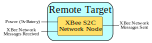
\includegraphics[scale=0.9]{figs/remote_target_block_diagram}
  \caption{Remote Target block diagram}
  \label{fig:remote_block_diag}
\end{figure}

\begin{figure}[h!]
  \centering
  \includegraphics[scale=0.82]{figs/mobile_cart_block_diagram}
  \caption{Block diagram showing the subsystem-level components of the proposed robotic cart.}
  \label{fig:mobile_block_diag}
\end{figure}

\subsection{System Components}
There are several components that are required for the mobile cart system. Although some of these parts are available in the Bradley University laboratory, other parts must be purchased. The parts that exist in the lab are shown in \autoref{tab:Partslablist}. Also, \autoref{tab:Partslist} shows the list of parts that we must purchase. The parts lists shown are the parts needed to build two mobile cart systems.

\begin{table}[h!]
  \centering
  \begin{tabular}{c|c}
      \toprule
      \textbf{Quantity} & \textbf{Parts}\\
      \toprule
      2 & Budget Bot Chassis\\
      4 & 10 uF Ceramic Capacitor\\
      4 & LM1117 Regulator\\
      2 & Battery Packs for Budget Bot\\
      8 & 9V Batteries\\
      4 & Solderable PCB Boards\\
      3 & XBee USB Adapter\\
      \bottomrule
      %\multicolumn{2}{r|}{\textbf{Total}} & \$ 562.34\\
      %\bottomrule
  \end{tabular}
  \caption{Parts Available in Laboratory}
  \label{tab:Partslablist}
\end{table}

\begin{table}[h!]
  \centering
  \begin{tabular}{c|c|c}
    \toprule
    \textbf{Quantity} & \textbf{Parts} & \textbf{Price}\\
    \toprule
    4 & Pololu 37D Metal Gear motor 4751 & \$ 39.95\\
    12 & XBee S2C Module & \$ 23.10\\
    10 & XBee Adapter Board & \$ 4.99\\
    2 & Twotrees 4 Lead Nema 17 Stepper Motor & \$ 9.99\\
    1 & 4-Pin JST SH Connector - 20 Pack & \$ 7.99\\
    1 & 6-Pin JST SH Connector - 10 Pack & \$ 9.99\\
    1 & Aluminum Foil Tape - 2 in x 5 yd & \$ 6.05\\
    \bottomrule
    \multicolumn{2}{r|}{\textbf{Total}} & \$ 562.34\\
    \bottomrule
  \end{tabular}
  \caption{Purchased parts for the Robotic Cart Project}
  \label{tab:Partslist}
\end{table}

\vspace*{12pt}
\noindent
The main components for this project are the Budget Bot Chassis (\autoref{fig:budgetBotChassis}), the BeagleBone Blue embedded computer (\autoref{fig:beagleboneBlue}), and the XBee S2C Modules (\autoref{fig:XBeeModule}). Another major component is the reflector array that
will be used to directionalize the RF signals received from the remote target that is with the user.

\begin{figure}
  \centering
  \begin{minipage}[t]{0.32\textwidth}
    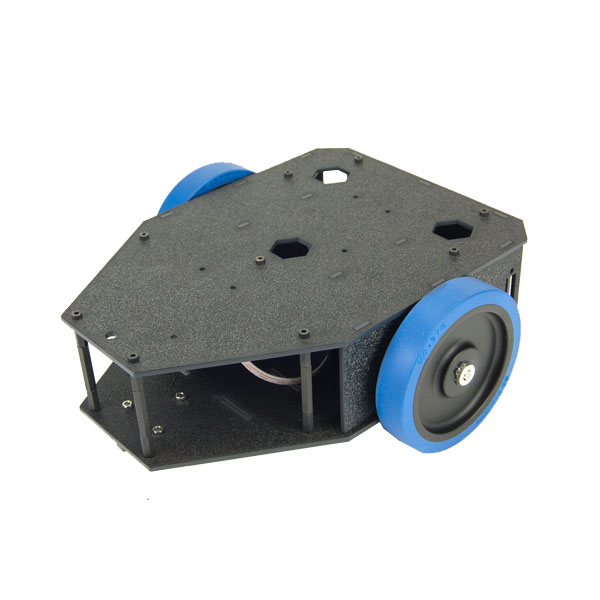
\includegraphics[width=1\textwidth]{figs/img/budgetbot_chassis}
    \captionsetup{width=\textwidth}
    \caption{Budget Bot Chassis}
    \label{fig:budgetBotChassis}
  \end{minipage}%
  \begin{minipage}[t]{0.32\textwidth}
    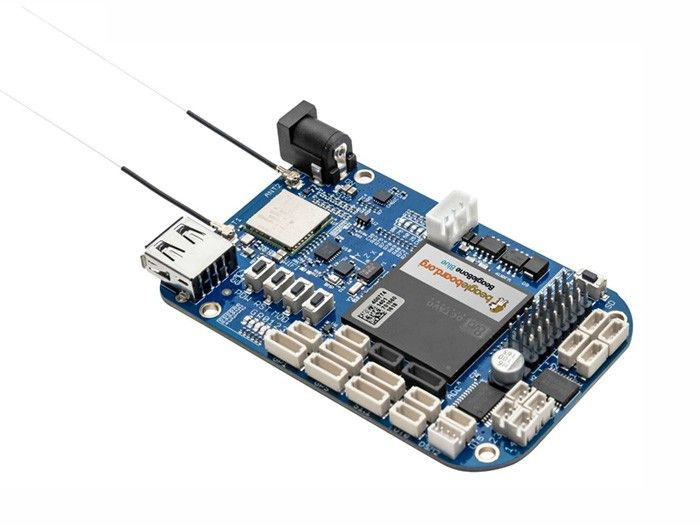
\includegraphics[width=1\textwidth]{figs/img/beaglebone_blue}
    \captionsetup{width=\textwidth}
    \caption{BeagleBone Blue}
    \label{fig:beagleboneBlue}
  \end{minipage}
  \begin{minipage}[t]{0.32\textwidth}
    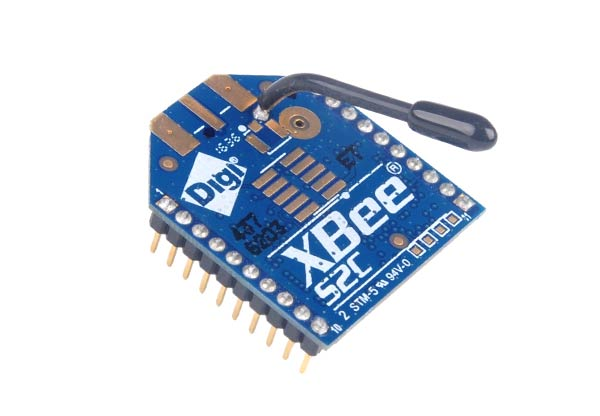
\includegraphics[width=1\textwidth]{figs/img/Xbee-S2C-Module}
    \captionsetup{width=\textwidth}
    \caption{XBee S2C Module}
    \label{fig:XBeeModule}
  \end{minipage}
\end{figure}

\vspace*{12pt}
\noindent
The reflector array will be mounted on top of the cart where it will be attached with a stepper motor. There are two reflector designs that we will be evaluating in this project. The first, shown in \autoref{fig:parabolodialReflector}, is a paraboloidal reflector which maximizes the signal strength of signals that come into the reflector directly perpendicularly. Since the remote will be carried by the user, it is likely that it will be positioned at a higher altitude than the reflector array. The paraboloidal reflector design may not be able to pick up the signals from the remote as well because of this. To solve this problem, we designed a combination parabolic/paraboloidal reflector, as shown in \autoref{fig:parabolicReflector}. The lower half of this reflector is paraboloidal in shape to limit the signals coming from below. The upper part of the reflector is strictly parabolic. This shape focuses the signals in the horizontal plane, but allows signals from above to still be received. We plan to construct both of these reflector designs by 3d printing the frames, then lining them with reflective foil tape. Both models will then be tested to determine which design works better.

\begin{figure}[h!]
  \centering
  \begin{minipage}[t]{0.5\textwidth}
    \centering
    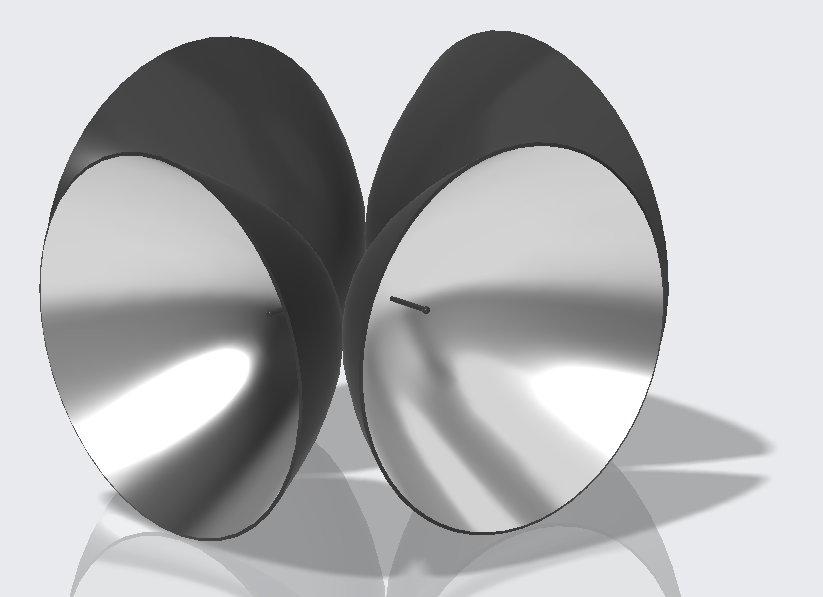
\includegraphics[height=2in]{figs/img/paraboloidalReflector}
    \captionsetup{width=\textwidth, justification=raggedright}
    \caption{Paraboloidal Reflector Model}
    \label{fig:parabolodialReflector}
  \end{minipage}
  \begin{minipage}[t]{0.4\textwidth}
    \centering
    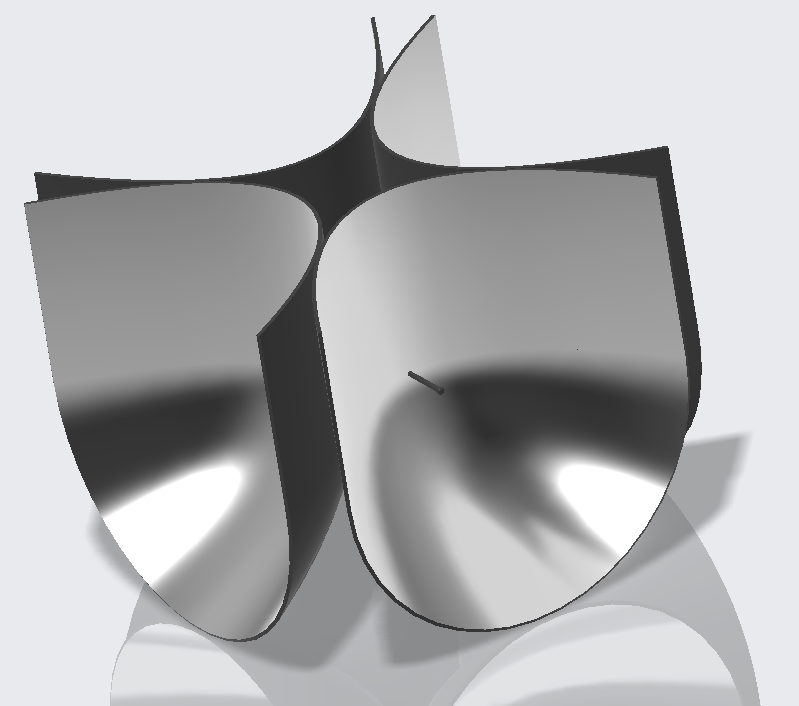
\includegraphics[height=2in]{figs/img/parabolicReflector}
    \captionsetup{width=\textwidth, justification=raggedright}
    \caption{Combined Parabolic/Paraboloidal Reflector}
    \label{fig:parabolicReflector}
  \end{minipage}
\end{figure}

\subsection{Operation of Mobile Cart System}
The Mobile Cart will controlled by a central embedded computer which we are using the BeagleBone Blue for. Two DC motors will be used to drive wheels to move the cart. Five XBee modules will be used to allow communication with the remote target. One of these radio sensors will be mounted on top of the cart to broadcast in all directions. The other four sensors will be placed inside parabolic reflectors at right angles to each other. This sensor array will be mounted on a stepper motor to allow rotation.

\vspace*{12pt}
\noindent
There are two main steps in the operation of the robotic cart system. The first step is localization of the remote in the robot's local coordinate frame. Once the location of the remote is known, the navigation step handles the control of the wheel velocities to move the cart to the desired location. A flowchart of the system operation is shown in \autoref{fig:sysOpFlowchart}.

\begin{figure}
  \centering
  % Graphic for TeX using PGF
% Title: S:\Senior Project\seniorProject2-2020-21-Docs\figs\dia\systemOperationFlowchart.dia
% Creator: Dia v0.97.2
% CreationDate: Wed Nov 25 16:20:30 2020
% For: Jason Braker
% \usepackage{tikz}
% The following commands are not supported in PSTricks at present
% We define them conditionally, so when they are implemented,
% this pgf file will use them.
\ifx\du\undefined
  \newlength{\du}
\fi
\setlength{\du}{15\unitlength}
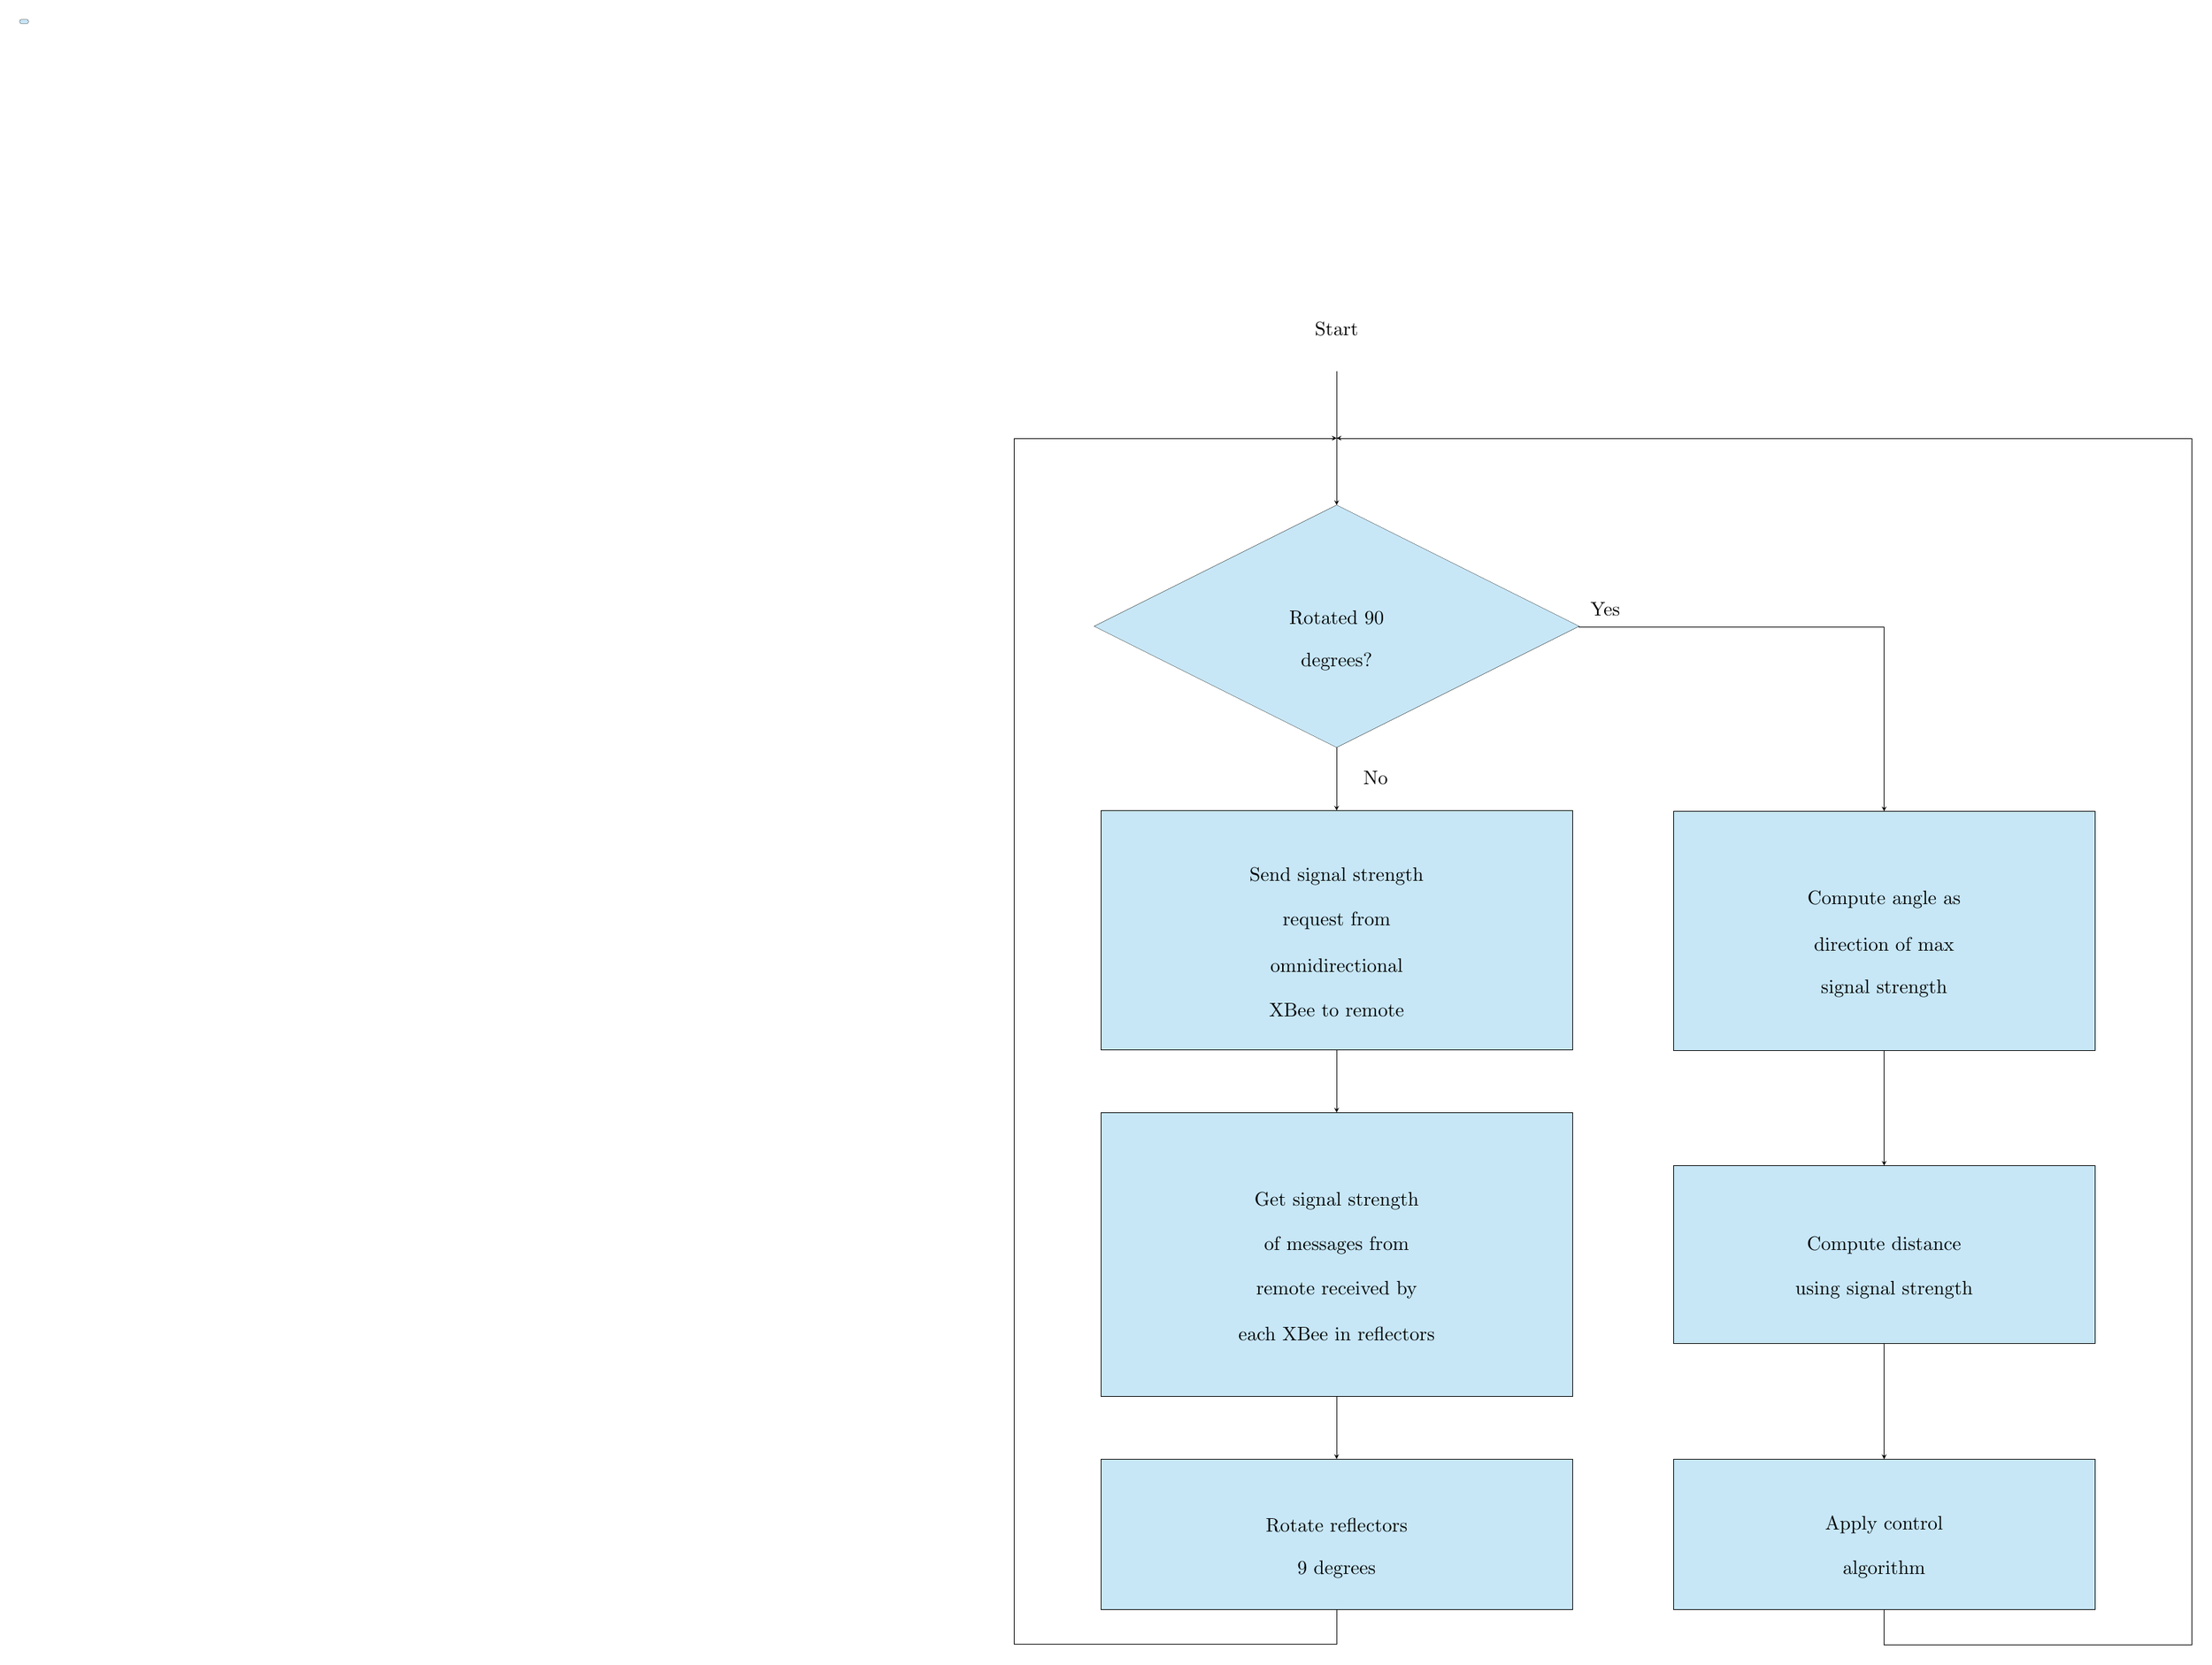
\begin{tikzpicture}
\pgftransformxscale{1.000000}
\pgftransformyscale{-1.000000}
\definecolor{dialinecolor}{rgb}{0.000000, 0.000000, 0.000000}
\pgfsetstrokecolor{dialinecolor}
\definecolor{dialinecolor}{rgb}{1.000000, 1.000000, 1.000000}
\pgfsetfillcolor{dialinecolor}
\pgfsetlinewidth{0.100000\du}
\pgfsetdash{}{0pt}
\pgfsetdash{}{0pt}
\pgfsetbuttcap
\pgfsetmiterjoin
\pgfsetlinewidth{0.100000\du}
\pgfsetbuttcap
\pgfsetmiterjoin
\pgfsetdash{}{0pt}
\definecolor{dialinecolor}{rgb}{0.780392, 0.905882, 0.968627}
\pgfsetfillcolor{dialinecolor}
\pgfpathmoveto{\pgfpoint{22.956946\du}{4.485162\du}}
\pgfpathlineto{\pgfpoint{25.983196\du}{4.485162\du}}
\pgfpathcurveto{\pgfpoint{26.401035\du}{4.485162\du}}{\pgfpoint{26.739759\du}{4.932877\du}}{\pgfpoint{26.739759\du}{5.485162\du}}
\pgfpathcurveto{\pgfpoint{26.739759\du}{6.037447\du}}{\pgfpoint{26.401035\du}{6.485162\du}}{\pgfpoint{25.983196\du}{6.485162\du}}
\pgfpathlineto{\pgfpoint{22.956946\du}{6.485162\du}}
\pgfpathcurveto{\pgfpoint{22.539108\du}{6.485162\du}}{\pgfpoint{22.200384\du}{6.037447\du}}{\pgfpoint{22.200384\du}{5.485162\du}}
\pgfpathcurveto{\pgfpoint{22.200384\du}{4.932877\du}}{\pgfpoint{22.539108\du}{4.485162\du}}{\pgfpoint{22.956946\du}{4.485162\du}}
\pgfusepath{fill}
\definecolor{dialinecolor}{rgb}{0.000000, 0.000000, 0.000000}
\pgfsetstrokecolor{dialinecolor}
\pgfpathmoveto{\pgfpoint{22.956946\du}{4.485162\du}}
\pgfpathlineto{\pgfpoint{25.983196\du}{4.485162\du}}
\pgfpathcurveto{\pgfpoint{26.401035\du}{4.485162\du}}{\pgfpoint{26.739759\du}{4.932877\du}}{\pgfpoint{26.739759\du}{5.485162\du}}
\pgfpathcurveto{\pgfpoint{26.739759\du}{6.037447\du}}{\pgfpoint{26.401035\du}{6.485162\du}}{\pgfpoint{25.983196\du}{6.485162\du}}
\pgfpathlineto{\pgfpoint{22.956946\du}{6.485162\du}}
\pgfpathcurveto{\pgfpoint{22.539108\du}{6.485162\du}}{\pgfpoint{22.200384\du}{6.037447\du}}{\pgfpoint{22.200384\du}{5.485162\du}}
\pgfpathcurveto{\pgfpoint{22.200384\du}{4.932877\du}}{\pgfpoint{22.539108\du}{4.485162\du}}{\pgfpoint{22.956946\du}{4.485162\du}}
\pgfusepath{stroke}
% setfont left to latex
\definecolor{dialinecolor}{rgb}{0.000000, 0.000000, 0.000000}
\pgfsetstrokecolor{dialinecolor}
\node at (24.470071\du,5.725162\du){Start};
\pgfsetlinewidth{0.100000\du}
\pgfsetdash{}{0pt}
\pgfsetdash{}{0pt}
\pgfsetbuttcap
{
\definecolor{dialinecolor}{rgb}{0.000000, 0.000000, 0.000000}
\pgfsetfillcolor{dialinecolor}
% was here!!!
\pgfsetarrowsend{stealth}
\definecolor{dialinecolor}{rgb}{0.000000, 0.000000, 0.000000}
\pgfsetstrokecolor{dialinecolor}
\draw (24.470071\du,13.253697\du)--(24.470071\du,14.388015\du);
}
\pgfsetlinewidth{0.100000\du}
\pgfsetdash{}{0pt}
\pgfsetdash{}{0pt}
\pgfsetbuttcap
{
\definecolor{dialinecolor}{rgb}{0.000000, 0.000000, 0.000000}
\pgfsetfillcolor{dialinecolor}
% was here!!!
\pgfsetarrowsend{stealth}
\definecolor{dialinecolor}{rgb}{0.000000, 0.000000, 0.000000}
\pgfsetstrokecolor{dialinecolor}
\draw (24.470071\du,6.485162\du)--(24.470071\du,8.891787\du);
}
\pgfsetlinewidth{0.100000\du}
\pgfsetdash{}{0pt}
\pgfsetdash{}{0pt}
\pgfsetmiterjoin
\pgfsetbuttcap
{
\definecolor{dialinecolor}{rgb}{0.000000, 0.000000, 0.000000}
\pgfsetfillcolor{dialinecolor}
% was here!!!
\pgfsetarrowsend{stealth}
{\pgfsetcornersarced{\pgfpoint{0.000000\du}{0.000000\du}}\definecolor{dialinecolor}{rgb}{0.000000, 0.000000, 0.000000}
\pgfsetstrokecolor{dialinecolor}
\draw (24.470071\du,28.756650\du)--(24.470071\du,29.380791\du)--(18.662017\du,29.380791\du)--(18.662017\du,7.688475\du)--(24.470071\du,7.688475\du);
}}
\pgfsetlinewidth{0.100000\du}
\pgfsetdash{}{0pt}
\pgfsetdash{}{0pt}
\pgfsetmiterjoin
\pgfsetbuttcap
{
\definecolor{dialinecolor}{rgb}{0.000000, 0.000000, 0.000000}
\pgfsetfillcolor{dialinecolor}
% was here!!!
\pgfsetarrowsend{stealth}
{\pgfsetcornersarced{\pgfpoint{0.000000\du}{0.000000\du}}\definecolor{dialinecolor}{rgb}{0.000000, 0.000000, 0.000000}
\pgfsetstrokecolor{dialinecolor}
\draw (28.831982\du,11.072742\du)--(28.831982\du,11.079441\du)--(34.317833\du,11.079441\du)--(34.317833\du,14.401811\du);
}}
% setfont left to latex
\definecolor{dialinecolor}{rgb}{0.000000, 0.000000, 0.000000}
\pgfsetstrokecolor{dialinecolor}
\node[anchor=west] at (28.920363\du,10.765993\du){Yes};
% setfont left to latex
\definecolor{dialinecolor}{rgb}{0.000000, 0.000000, 0.000000}
\pgfsetstrokecolor{dialinecolor}
\node[anchor=west] at (24.833774\du,13.804637\du){No};
\definecolor{dialinecolor}{rgb}{0.780392, 0.905882, 0.968627}
\pgfsetfillcolor{dialinecolor}
\fill (20.230538\du,19.822333\du)--(20.230538\du,24.922333\du)--(28.709605\du,24.922333\du)--(28.709605\du,19.822333\du)--cycle;
\pgfsetlinewidth{0.100000\du}
\pgfsetdash{}{0pt}
\pgfsetdash{}{0pt}
\pgfsetmiterjoin
\definecolor{dialinecolor}{rgb}{0.000000, 0.000000, 0.000000}
\pgfsetstrokecolor{dialinecolor}
\draw (20.230538\du,19.822333\du)--(20.230538\du,24.922333\du)--(28.709605\du,24.922333\du)--(28.709605\du,19.822333\du)--cycle;
% setfont left to latex
\definecolor{dialinecolor}{rgb}{0.000000, 0.000000, 0.000000}
\pgfsetstrokecolor{dialinecolor}
\node at (24.470071\du,21.412333\du){Get signal strength};
% setfont left to latex
\definecolor{dialinecolor}{rgb}{0.000000, 0.000000, 0.000000}
\pgfsetstrokecolor{dialinecolor}
\node at (24.470071\du,22.212333\du){of messages from};
% setfont left to latex
\definecolor{dialinecolor}{rgb}{0.000000, 0.000000, 0.000000}
\pgfsetstrokecolor{dialinecolor}
\node at (24.470071\du,23.012333\du){remote received by};
% setfont left to latex
\definecolor{dialinecolor}{rgb}{0.000000, 0.000000, 0.000000}
\pgfsetstrokecolor{dialinecolor}
\node at (24.470071\du,23.812333\du){each XBee in reflectors};
\definecolor{dialinecolor}{rgb}{0.780392, 0.905882, 0.968627}
\pgfsetfillcolor{dialinecolor}
\fill (24.470071\du,8.891787\du)--(28.831982\du,11.072742\du)--(24.470071\du,13.253697\du)--(20.108161\du,11.072742\du)--cycle;
\pgfsetlinewidth{0.100000\du}
\pgfsetdash{}{0pt}
\pgfsetdash{}{0pt}
\pgfsetmiterjoin
\definecolor{dialinecolor}{rgb}{0.000000, 0.000000, 0.000000}
\pgfsetstrokecolor{dialinecolor}
\draw (24.470071\du,8.891787\du)--(28.831982\du,11.072742\du)--(24.470071\du,13.253697\du)--(20.108161\du,11.072742\du)--cycle;
% setfont left to latex
\definecolor{dialinecolor}{rgb}{0.000000, 0.000000, 0.000000}
\pgfsetstrokecolor{dialinecolor}
\node at (24.470071\du,10.912742\du){Rotated 90};
% setfont left to latex
\definecolor{dialinecolor}{rgb}{0.000000, 0.000000, 0.000000}
\pgfsetstrokecolor{dialinecolor}
\node at (24.470071\du,11.712742\du){degrees?};
\definecolor{dialinecolor}{rgb}{0.780392, 0.905882, 0.968627}
\pgfsetfillcolor{dialinecolor}
\fill (30.525333\du,14.401811\du)--(30.525333\du,18.701811\du)--(38.110333\du,18.701811\du)--(38.110333\du,14.401811\du)--cycle;
\pgfsetlinewidth{0.100000\du}
\pgfsetdash{}{0pt}
\pgfsetdash{}{0pt}
\pgfsetmiterjoin
\definecolor{dialinecolor}{rgb}{0.000000, 0.000000, 0.000000}
\pgfsetstrokecolor{dialinecolor}
\draw (30.525333\du,14.401811\du)--(30.525333\du,18.701811\du)--(38.110333\du,18.701811\du)--(38.110333\du,14.401811\du)--cycle;
% setfont left to latex
\definecolor{dialinecolor}{rgb}{0.000000, 0.000000, 0.000000}
\pgfsetstrokecolor{dialinecolor}
\node at (34.317833\du,15.991811\du){Compute angle as};
% setfont left to latex
\definecolor{dialinecolor}{rgb}{0.000000, 0.000000, 0.000000}
\pgfsetstrokecolor{dialinecolor}
\node at (34.317833\du,16.791811\du){direction of max};
% setfont left to latex
\definecolor{dialinecolor}{rgb}{0.000000, 0.000000, 0.000000}
\pgfsetstrokecolor{dialinecolor}
\node at (34.317833\du,17.591811\du){signal strength};
\definecolor{dialinecolor}{rgb}{0.780392, 0.905882, 0.968627}
\pgfsetfillcolor{dialinecolor}
\fill (30.525333\du,20.777419\du)--(30.525333\du,23.968519\du)--(38.110333\du,23.968519\du)--(38.110333\du,20.777419\du)--cycle;
\pgfsetlinewidth{0.100000\du}
\pgfsetdash{}{0pt}
\pgfsetdash{}{0pt}
\pgfsetmiterjoin
\definecolor{dialinecolor}{rgb}{0.000000, 0.000000, 0.000000}
\pgfsetstrokecolor{dialinecolor}
\draw (30.525333\du,20.777419\du)--(30.525333\du,23.968519\du)--(38.110333\du,23.968519\du)--(38.110333\du,20.777419\du)--cycle;
% setfont left to latex
\definecolor{dialinecolor}{rgb}{0.000000, 0.000000, 0.000000}
\pgfsetstrokecolor{dialinecolor}
\node at (34.317833\du,22.212969\du){Compute distance};
% setfont left to latex
\definecolor{dialinecolor}{rgb}{0.000000, 0.000000, 0.000000}
\pgfsetstrokecolor{dialinecolor}
\node at (34.317833\du,23.012969\du){using signal strength};
\definecolor{dialinecolor}{rgb}{0.780392, 0.905882, 0.968627}
\pgfsetfillcolor{dialinecolor}
\fill (30.525333\du,26.058941\du)--(30.525333\du,28.758941\du)--(38.110333\du,28.758941\du)--(38.110333\du,26.058941\du)--cycle;
\pgfsetlinewidth{0.100000\du}
\pgfsetdash{}{0pt}
\pgfsetdash{}{0pt}
\pgfsetmiterjoin
\definecolor{dialinecolor}{rgb}{0.000000, 0.000000, 0.000000}
\pgfsetstrokecolor{dialinecolor}
\draw (30.525333\du,26.058941\du)--(30.525333\du,28.758941\du)--(38.110333\du,28.758941\du)--(38.110333\du,26.058941\du)--cycle;
% setfont left to latex
\definecolor{dialinecolor}{rgb}{0.000000, 0.000000, 0.000000}
\pgfsetstrokecolor{dialinecolor}
\node at (34.317833\du,27.248941\du){Apply control};
% setfont left to latex
\definecolor{dialinecolor}{rgb}{0.000000, 0.000000, 0.000000}
\pgfsetstrokecolor{dialinecolor}
\node at (34.317833\du,28.048941\du){algorithm};
\pgfsetlinewidth{0.100000\du}
\pgfsetdash{}{0pt}
\pgfsetdash{}{0pt}
\pgfsetbuttcap
{
\definecolor{dialinecolor}{rgb}{0.000000, 0.000000, 0.000000}
\pgfsetfillcolor{dialinecolor}
% was here!!!
\pgfsetarrowsend{stealth}
\definecolor{dialinecolor}{rgb}{0.000000, 0.000000, 0.000000}
\pgfsetstrokecolor{dialinecolor}
\draw (24.470071\du,18.688015\du)--(24.470071\du,19.822333\du);
}
\pgfsetlinewidth{0.100000\du}
\pgfsetdash{}{0pt}
\pgfsetdash{}{0pt}
\pgfsetbuttcap
{
\definecolor{dialinecolor}{rgb}{0.000000, 0.000000, 0.000000}
\pgfsetfillcolor{dialinecolor}
% was here!!!
\pgfsetarrowsend{stealth}
\definecolor{dialinecolor}{rgb}{0.000000, 0.000000, 0.000000}
\pgfsetstrokecolor{dialinecolor}
\draw (24.470071\du,24.922333\du)--(24.470071\du,26.056650\du);
}
\pgfsetlinewidth{0.100000\du}
\pgfsetdash{}{0pt}
\pgfsetdash{}{0pt}
\pgfsetbuttcap
{
\definecolor{dialinecolor}{rgb}{0.000000, 0.000000, 0.000000}
\pgfsetfillcolor{dialinecolor}
% was here!!!
\pgfsetarrowsend{stealth}
\definecolor{dialinecolor}{rgb}{0.000000, 0.000000, 0.000000}
\pgfsetstrokecolor{dialinecolor}
\draw (34.317833\du,18.701811\du)--(34.317833\du,20.777419\du);
}
\pgfsetlinewidth{0.100000\du}
\pgfsetdash{}{0pt}
\pgfsetdash{}{0pt}
\pgfsetbuttcap
{
\definecolor{dialinecolor}{rgb}{0.000000, 0.000000, 0.000000}
\pgfsetfillcolor{dialinecolor}
% was here!!!
\pgfsetarrowsend{stealth}
\definecolor{dialinecolor}{rgb}{0.000000, 0.000000, 0.000000}
\pgfsetstrokecolor{dialinecolor}
\draw (34.317833\du,23.968519\du)--(34.317833\du,26.058941\du);
}
\pgfsetlinewidth{0.100000\du}
\pgfsetdash{}{0pt}
\pgfsetdash{}{0pt}
\pgfsetmiterjoin
\pgfsetbuttcap
{
\definecolor{dialinecolor}{rgb}{0.000000, 0.000000, 0.000000}
\pgfsetfillcolor{dialinecolor}
% was here!!!
\pgfsetarrowsend{stealth}
{\pgfsetcornersarced{\pgfpoint{0.000000\du}{0.000000\du}}\definecolor{dialinecolor}{rgb}{0.000000, 0.000000, 0.000000}
\pgfsetstrokecolor{dialinecolor}
\draw (34.317833\du,28.758941\du)--(34.317833\du,29.400791\du)--(39.852453\du,29.400791\du)--(39.852453\du,7.688475\du)--(24.470071\du,7.688475\du);
}}
\definecolor{dialinecolor}{rgb}{0.780392, 0.905882, 0.968627}
\pgfsetfillcolor{dialinecolor}
\fill (20.230538\du,14.388015\du)--(20.230538\du,18.688015\du)--(28.709605\du,18.688015\du)--(28.709605\du,14.388015\du)--cycle;
\pgfsetlinewidth{0.100000\du}
\pgfsetdash{}{0pt}
\pgfsetdash{}{0pt}
\pgfsetmiterjoin
\definecolor{dialinecolor}{rgb}{0.000000, 0.000000, 0.000000}
\pgfsetstrokecolor{dialinecolor}
\draw (20.230538\du,14.388015\du)--(20.230538\du,18.688015\du)--(28.709605\du,18.688015\du)--(28.709605\du,14.388015\du)--cycle;
% setfont left to latex
\definecolor{dialinecolor}{rgb}{0.000000, 0.000000, 0.000000}
\pgfsetstrokecolor{dialinecolor}
\node at (24.470071\du,15.578015\du){Send signal strength};
% setfont left to latex
\definecolor{dialinecolor}{rgb}{0.000000, 0.000000, 0.000000}
\pgfsetstrokecolor{dialinecolor}
\node at (24.470071\du,16.378015\du){request from};
% setfont left to latex
\definecolor{dialinecolor}{rgb}{0.000000, 0.000000, 0.000000}
\pgfsetstrokecolor{dialinecolor}
\node at (24.470071\du,17.178015\du){omnidirectional};
% setfont left to latex
\definecolor{dialinecolor}{rgb}{0.000000, 0.000000, 0.000000}
\pgfsetstrokecolor{dialinecolor}
\node at (24.470071\du,17.978015\du){XBee to remote};
\definecolor{dialinecolor}{rgb}{0.780392, 0.905882, 0.968627}
\pgfsetfillcolor{dialinecolor}
\fill (20.230538\du,26.056650\du)--(20.230538\du,28.756650\du)--(28.709605\du,28.756650\du)--(28.709605\du,26.056650\du)--cycle;
\pgfsetlinewidth{0.100000\du}
\pgfsetdash{}{0pt}
\pgfsetdash{}{0pt}
\pgfsetmiterjoin
\definecolor{dialinecolor}{rgb}{0.000000, 0.000000, 0.000000}
\pgfsetstrokecolor{dialinecolor}
\draw (20.230538\du,26.056650\du)--(20.230538\du,28.756650\du)--(28.709605\du,28.756650\du)--(28.709605\du,26.056650\du)--cycle;
% setfont left to latex
\definecolor{dialinecolor}{rgb}{0.000000, 0.000000, 0.000000}
\pgfsetstrokecolor{dialinecolor}
\node at (24.470071\du,27.246650\du){Rotate reflectors};
% setfont left to latex
\definecolor{dialinecolor}{rgb}{0.000000, 0.000000, 0.000000}
\pgfsetstrokecolor{dialinecolor}
\node at (24.470071\du,28.046650\du){9 degrees};
\end{tikzpicture}

  \caption{Flowchart of System Operation}
  \label{fig:sysOpFlowchart}
\end{figure}

\subsection{Algorithms}
As mentioned previously, there are two steps in the operation of the system. These steps are the localization of the remote and the navigation of the robot. This section describes the algorithms used for these tasks.

\subsubsection{Localization Algorithm}
The strength of the radio signals between the cart and remote will be used to estimate the position of the remote relative to the cart. By rotating the sensor array 90 degrees and measuring the signal strength of messages from the remote at several steps in the rotation, the bearing of the remote can be estimated as the direction in which the maximum signal strength is received. To estimate the distance between the cart and the remote, the signal strength will be measured and used to calculate the distance. The omnidirectional radio module on top will be responsible for coordinating the messages from the remote by sending the remote commands that tell the remote when to send signals. A flowchart of the localization algorithm is shown in \autoref{fig:locAlgoFlowchart}. Also, a pseudo-code version of the algorithm is shown in \autoref{alg:locAlgo}

\begin{figure}
  \centering
  % Graphic for TeX using PGF
% Title: S:\Senior Project\seniorProject2-2020-21-Docs\figs\dia\systemOperationFlowchart.dia
% Creator: Dia v0.97.2
% CreationDate: Tue Dec 01 10:06:16 2020
% For: Jason Braker
% \usepackage{tikz}
% The following commands are not supported in PSTricks at present
% We define them conditionally, so when they are implemented,
% this pgf file will use them.
\ifx\du\undefined
  \newlength{\du}
\fi
\setlength{\du}{15\unitlength}
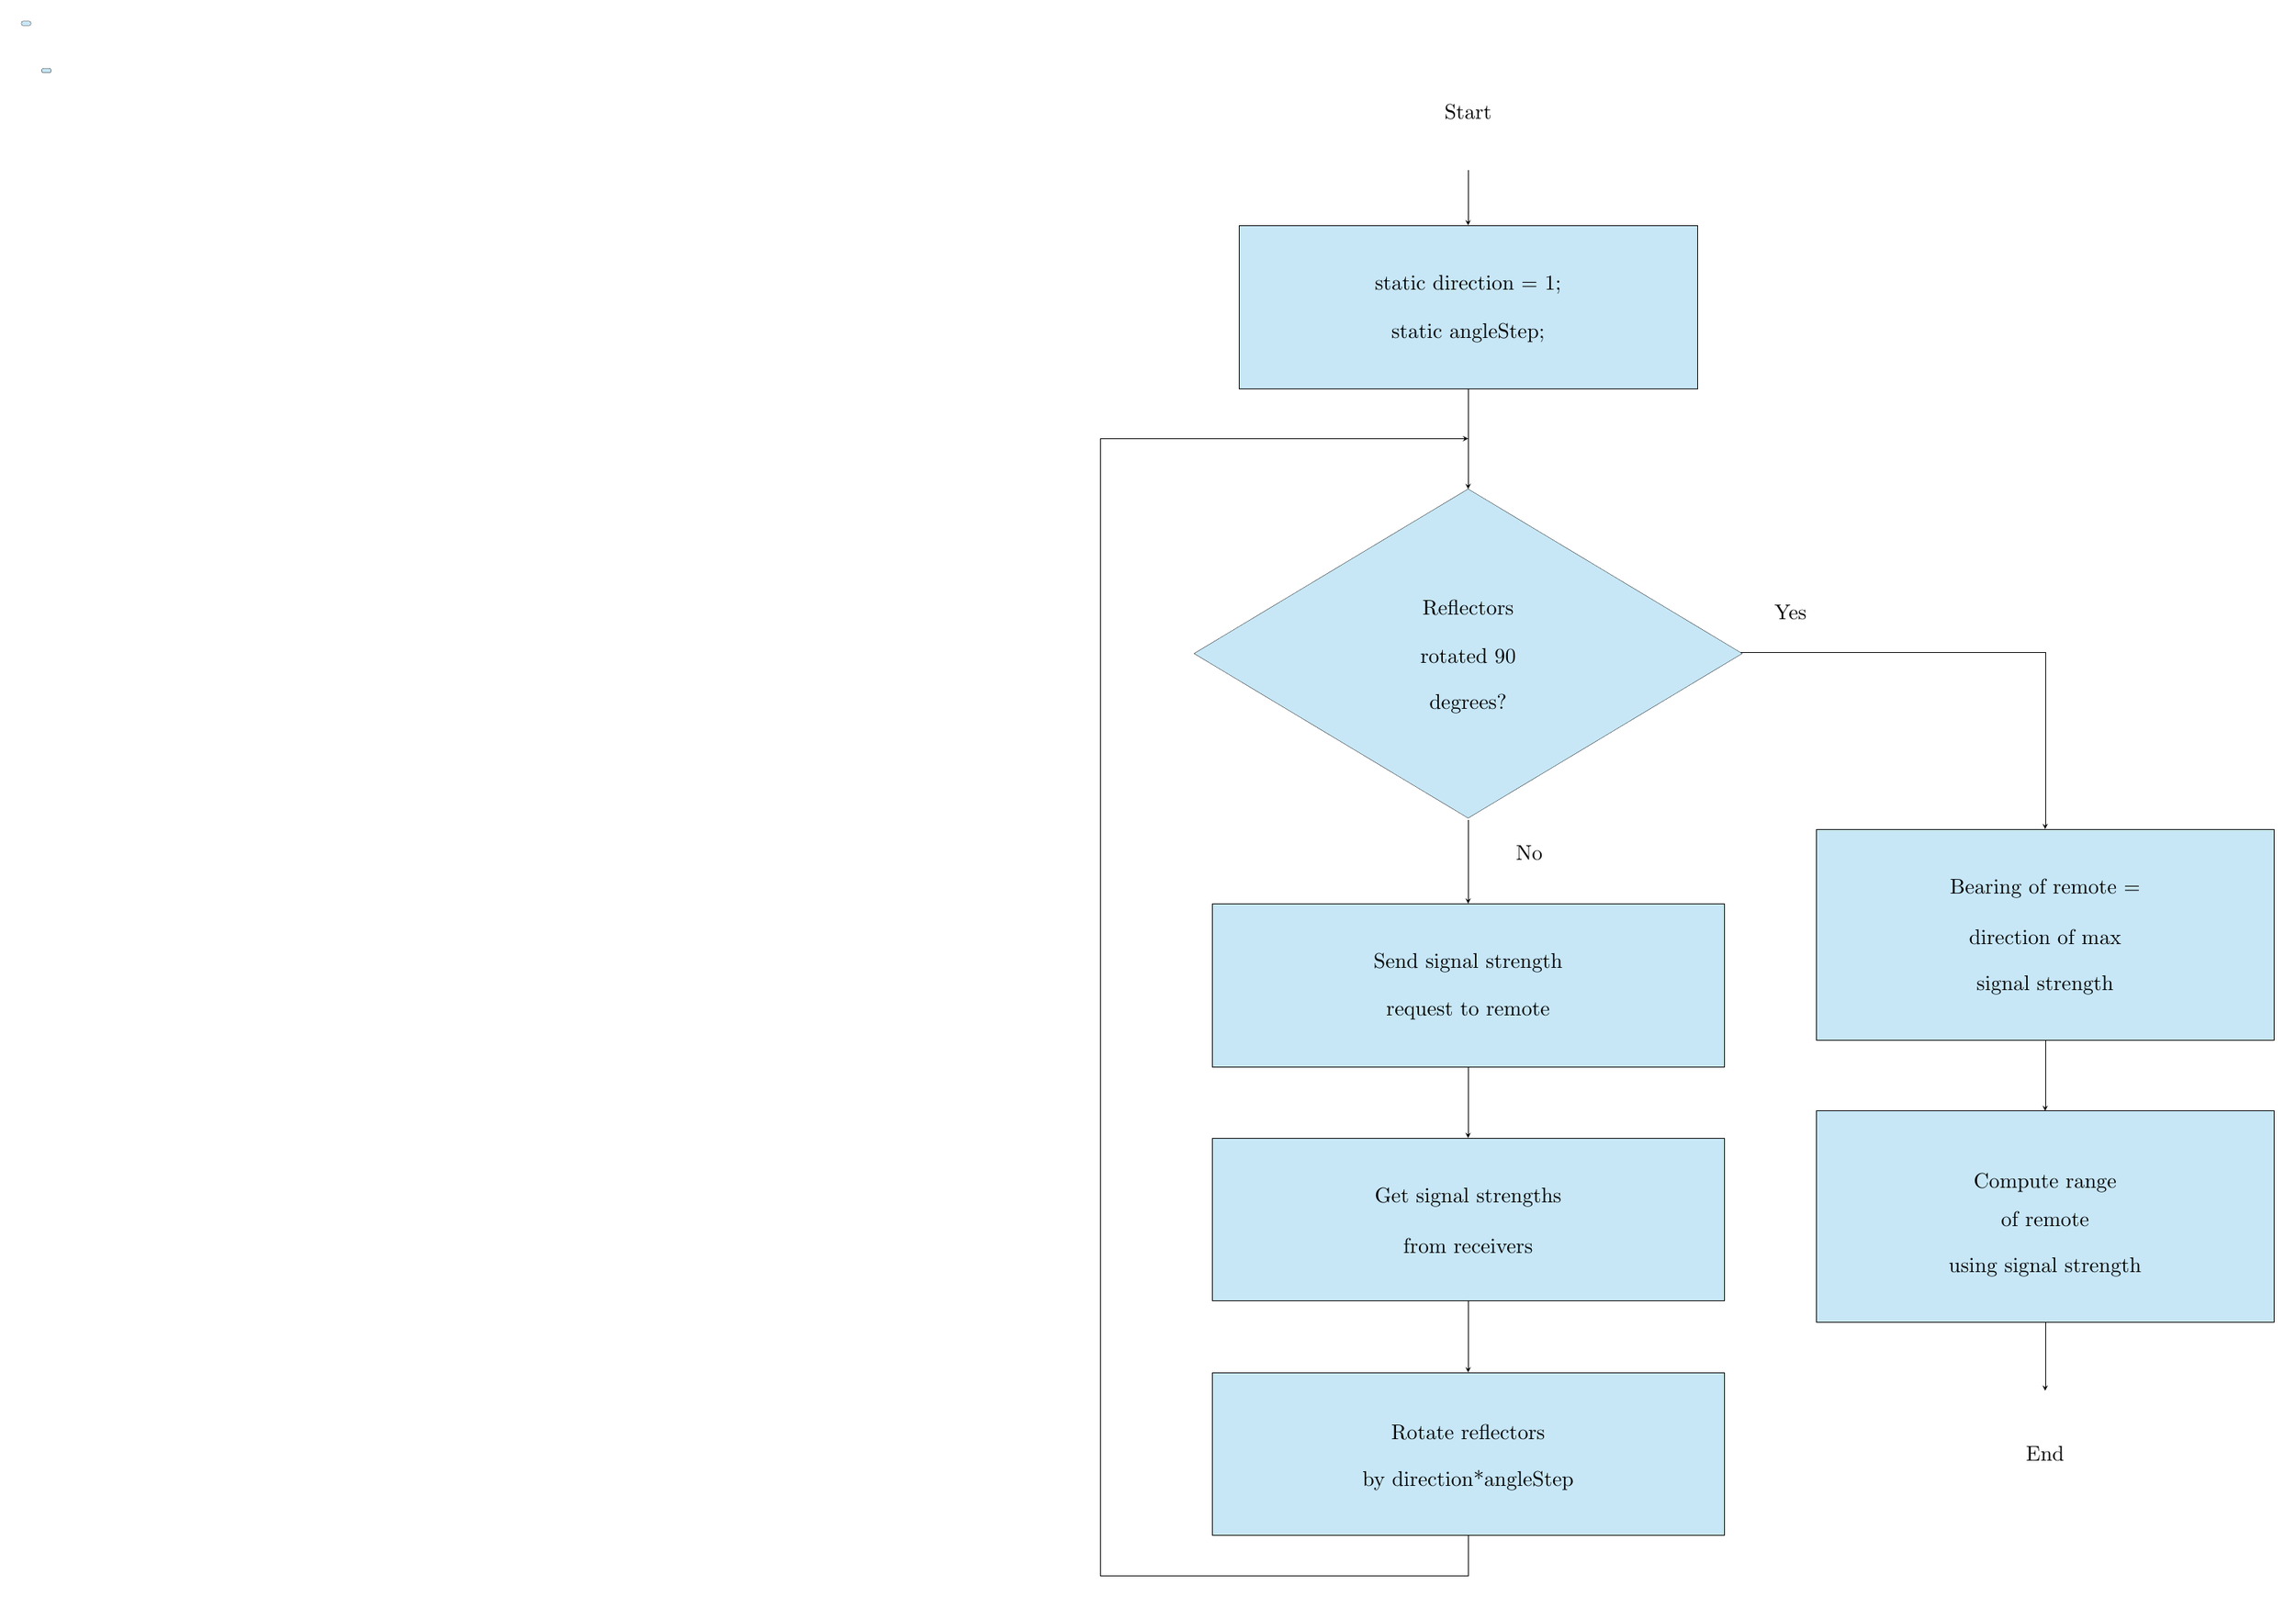
\begin{tikzpicture}
\pgftransformxscale{1.000000}
\pgftransformyscale{-1.000000}
\definecolor{dialinecolor}{rgb}{0.000000, 0.000000, 0.000000}
\pgfsetstrokecolor{dialinecolor}
\definecolor{dialinecolor}{rgb}{1.000000, 1.000000, 1.000000}
\pgfsetfillcolor{dialinecolor}
\pgfsetlinewidth{0.100000\du}
\pgfsetdash{}{0pt}
\pgfsetdash{}{0pt}
\pgfsetbuttcap
\pgfsetmiterjoin
\pgfsetlinewidth{0.100000\du}
\pgfsetbuttcap
\pgfsetmiterjoin
\pgfsetdash{}{0pt}
\definecolor{dialinecolor}{rgb}{0.780392, 0.905882, 0.968627}
\pgfsetfillcolor{dialinecolor}
\pgfpathmoveto{\pgfpoint{23.245553\du}{0.476720\du}}
\pgfpathlineto{\pgfpoint{26.271803\du}{0.476720\du}}
\pgfpathcurveto{\pgfpoint{26.689641\du}{0.476720\du}}{\pgfpoint{27.028366\du}{0.924435\du}}{\pgfpoint{27.028366\du}{1.476720\du}}
\pgfpathcurveto{\pgfpoint{27.028366\du}{2.029005\du}}{\pgfpoint{26.689641\du}{2.476720\du}}{\pgfpoint{26.271803\du}{2.476720\du}}
\pgfpathlineto{\pgfpoint{23.245553\du}{2.476720\du}}
\pgfpathcurveto{\pgfpoint{22.827715\du}{2.476720\du}}{\pgfpoint{22.488991\du}{2.029005\du}}{\pgfpoint{22.488991\du}{1.476720\du}}
\pgfpathcurveto{\pgfpoint{22.488991\du}{0.924435\du}}{\pgfpoint{22.827715\du}{0.476720\du}}{\pgfpoint{23.245553\du}{0.476720\du}}
\pgfusepath{fill}
\definecolor{dialinecolor}{rgb}{0.000000, 0.000000, 0.000000}
\pgfsetstrokecolor{dialinecolor}
\pgfpathmoveto{\pgfpoint{23.245553\du}{0.476720\du}}
\pgfpathlineto{\pgfpoint{26.271803\du}{0.476720\du}}
\pgfpathcurveto{\pgfpoint{26.689641\du}{0.476720\du}}{\pgfpoint{27.028366\du}{0.924435\du}}{\pgfpoint{27.028366\du}{1.476720\du}}
\pgfpathcurveto{\pgfpoint{27.028366\du}{2.029005\du}}{\pgfpoint{26.689641\du}{2.476720\du}}{\pgfpoint{26.271803\du}{2.476720\du}}
\pgfpathlineto{\pgfpoint{23.245553\du}{2.476720\du}}
\pgfpathcurveto{\pgfpoint{22.827715\du}{2.476720\du}}{\pgfpoint{22.488991\du}{2.029005\du}}{\pgfpoint{22.488991\du}{1.476720\du}}
\pgfpathcurveto{\pgfpoint{22.488991\du}{0.924435\du}}{\pgfpoint{22.827715\du}{0.476720\du}}{\pgfpoint{23.245553\du}{0.476720\du}}
\pgfusepath{stroke}
% setfont left to latex
\definecolor{dialinecolor}{rgb}{0.000000, 0.000000, 0.000000}
\pgfsetstrokecolor{dialinecolor}
\node at (24.758678\du,1.516720\du){Start};
\pgfsetlinewidth{0.100000\du}
\pgfsetdash{}{0pt}
\pgfsetdash{}{0pt}
\pgfsetbuttcap
{
\definecolor{dialinecolor}{rgb}{0.000000, 0.000000, 0.000000}
\pgfsetfillcolor{dialinecolor}
% was here!!!
\pgfsetarrowsend{stealth}
\definecolor{dialinecolor}{rgb}{0.000000, 0.000000, 0.000000}
\pgfsetstrokecolor{dialinecolor}
\draw (24.758678\du,13.254938\du)--(24.758678\du,14.638000\du);
}
\pgfsetlinewidth{0.100000\du}
\pgfsetdash{}{0pt}
\pgfsetdash{}{0pt}
\pgfsetbuttcap
{
\definecolor{dialinecolor}{rgb}{0.000000, 0.000000, 0.000000}
\pgfsetfillcolor{dialinecolor}
% was here!!!
\pgfsetarrowsend{stealth}
\definecolor{dialinecolor}{rgb}{0.000000, 0.000000, 0.000000}
\pgfsetstrokecolor{dialinecolor}
\draw (24.758678\du,6.097900\du)--(24.758678\du,7.767002\du);
}
\pgfsetlinewidth{0.100000\du}
\pgfsetdash{}{0pt}
\pgfsetdash{}{0pt}
\pgfsetmiterjoin
\pgfsetbuttcap
{
\definecolor{dialinecolor}{rgb}{0.000000, 0.000000, 0.000000}
\pgfsetfillcolor{dialinecolor}
% was here!!!
\pgfsetarrowsend{stealth}
{\pgfsetcornersarced{\pgfpoint{0.000000\du}{0.000000\du}}\definecolor{dialinecolor}{rgb}{0.000000, 0.000000, 0.000000}
\pgfsetstrokecolor{dialinecolor}
\draw (24.758678\du,25.106700\du)--(24.758678\du,25.775000\du)--(18.662000\du,25.775000\du)--(18.662000\du,6.932451\du)--(24.758678\du,6.932451\du);
}}
\pgfsetlinewidth{0.100000\du}
\pgfsetdash{}{0pt}
\pgfsetdash{}{0pt}
\pgfsetmiterjoin
\pgfsetbuttcap
{
\definecolor{dialinecolor}{rgb}{0.000000, 0.000000, 0.000000}
\pgfsetfillcolor{dialinecolor}
% was here!!!
\pgfsetarrowsend{stealth}
{\pgfsetcornersarced{\pgfpoint{0.000000\du}{0.000000\du}}\definecolor{dialinecolor}{rgb}{0.000000, 0.000000, 0.000000}
\pgfsetstrokecolor{dialinecolor}
\draw (29.260647\du,10.510970\du)--(29.260647\du,10.475000\du)--(34.317800\du,10.475000\du)--(34.317800\du,13.401800\du);
}}
% setfont left to latex
\definecolor{dialinecolor}{rgb}{0.000000, 0.000000, 0.000000}
\pgfsetstrokecolor{dialinecolor}
\node[anchor=west] at (29.716400\du,9.806400\du){Yes};
% setfont left to latex
\definecolor{dialinecolor}{rgb}{0.000000, 0.000000, 0.000000}
\pgfsetstrokecolor{dialinecolor}
\node[anchor=west] at (25.433800\du,13.804600\du){No};
\definecolor{dialinecolor}{rgb}{0.780392, 0.905882, 0.968627}
\pgfsetfillcolor{dialinecolor}
\fill (20.519144\du,18.522300\du)--(20.519144\du,21.222300\du)--(28.998212\du,21.222300\du)--(28.998212\du,18.522300\du)--cycle;
\pgfsetlinewidth{0.100000\du}
\pgfsetdash{}{0pt}
\pgfsetdash{}{0pt}
\pgfsetmiterjoin
\definecolor{dialinecolor}{rgb}{0.000000, 0.000000, 0.000000}
\pgfsetstrokecolor{dialinecolor}
\draw (20.519144\du,18.522300\du)--(20.519144\du,21.222300\du)--(28.998212\du,21.222300\du)--(28.998212\du,18.522300\du)--cycle;
% setfont left to latex
\definecolor{dialinecolor}{rgb}{0.000000, 0.000000, 0.000000}
\pgfsetstrokecolor{dialinecolor}
\node at (24.758678\du,19.512300\du){Get signal strengths};
% setfont left to latex
\definecolor{dialinecolor}{rgb}{0.000000, 0.000000, 0.000000}
\pgfsetstrokecolor{dialinecolor}
\node at (24.758678\du,20.312300\du){from receivers};
\definecolor{dialinecolor}{rgb}{0.780392, 0.905882, 0.968627}
\pgfsetfillcolor{dialinecolor}
\fill (24.758678\du,7.767002\du)--(29.299535\du,10.494358\du)--(24.758678\du,13.221715\du)--(20.217821\du,10.494358\du)--cycle;
\pgfsetlinewidth{0.100000\du}
\pgfsetdash{}{0pt}
\pgfsetdash{}{0pt}
\pgfsetmiterjoin
\definecolor{dialinecolor}{rgb}{0.000000, 0.000000, 0.000000}
\pgfsetstrokecolor{dialinecolor}
\draw (24.758678\du,7.767002\du)--(29.299535\du,10.494358\du)--(24.758678\du,13.221715\du)--(20.217821\du,10.494358\du)--cycle;
% setfont left to latex
\definecolor{dialinecolor}{rgb}{0.000000, 0.000000, 0.000000}
\pgfsetstrokecolor{dialinecolor}
\node at (24.758678\du,9.734358\du){Reflectors};
% setfont left to latex
\definecolor{dialinecolor}{rgb}{0.000000, 0.000000, 0.000000}
\pgfsetstrokecolor{dialinecolor}
\node at (24.758678\du,10.534358\du){rotated 90};
% setfont left to latex
\definecolor{dialinecolor}{rgb}{0.000000, 0.000000, 0.000000}
\pgfsetstrokecolor{dialinecolor}
\node at (24.758678\du,11.334358\du){degrees?};
\definecolor{dialinecolor}{rgb}{0.780392, 0.905882, 0.968627}
\pgfsetfillcolor{dialinecolor}
\fill (30.525300\du,13.401800\du)--(30.525300\du,16.901800\du)--(38.110300\du,16.901800\du)--(38.110300\du,13.401800\du)--cycle;
\pgfsetlinewidth{0.100000\du}
\pgfsetdash{}{0pt}
\pgfsetdash{}{0pt}
\pgfsetmiterjoin
\definecolor{dialinecolor}{rgb}{0.000000, 0.000000, 0.000000}
\pgfsetstrokecolor{dialinecolor}
\draw (30.525300\du,13.401800\du)--(30.525300\du,16.901800\du)--(38.110300\du,16.901800\du)--(38.110300\du,13.401800\du)--cycle;
% setfont left to latex
\definecolor{dialinecolor}{rgb}{0.000000, 0.000000, 0.000000}
\pgfsetstrokecolor{dialinecolor}
\node at (34.317800\du,14.391800\du){Bearing of remote =};
% setfont left to latex
\definecolor{dialinecolor}{rgb}{0.000000, 0.000000, 0.000000}
\pgfsetstrokecolor{dialinecolor}
\node at (34.317800\du,15.191800\du){direction of max};
% setfont left to latex
\definecolor{dialinecolor}{rgb}{0.000000, 0.000000, 0.000000}
\pgfsetstrokecolor{dialinecolor}
\node at (34.317800\du,15.991800\du){signal strength};
\definecolor{dialinecolor}{rgb}{0.780392, 0.905882, 0.968627}
\pgfsetfillcolor{dialinecolor}
\fill (30.525300\du,18.072900\du)--(30.525300\du,21.572900\du)--(38.110300\du,21.572900\du)--(38.110300\du,18.072900\du)--cycle;
\pgfsetlinewidth{0.100000\du}
\pgfsetdash{}{0pt}
\pgfsetdash{}{0pt}
\pgfsetmiterjoin
\definecolor{dialinecolor}{rgb}{0.000000, 0.000000, 0.000000}
\pgfsetstrokecolor{dialinecolor}
\draw (30.525300\du,18.072900\du)--(30.525300\du,21.572900\du)--(38.110300\du,21.572900\du)--(38.110300\du,18.072900\du)--cycle;
% setfont left to latex
\definecolor{dialinecolor}{rgb}{0.000000, 0.000000, 0.000000}
\pgfsetstrokecolor{dialinecolor}
\node at (34.317800\du,19.262900\du){Compute range};
% setfont left to latex
\definecolor{dialinecolor}{rgb}{0.000000, 0.000000, 0.000000}
\pgfsetstrokecolor{dialinecolor}
\node at (34.317800\du,19.862900\du){of remote};
% setfont left to latex
\definecolor{dialinecolor}{rgb}{0.000000, 0.000000, 0.000000}
\pgfsetstrokecolor{dialinecolor}
\node at (34.317800\du,20.662900\du){using signal strength};
\pgfsetlinewidth{0.100000\du}
\pgfsetdash{}{0pt}
\pgfsetdash{}{0pt}
\pgfsetbuttcap
{
\definecolor{dialinecolor}{rgb}{0.000000, 0.000000, 0.000000}
\pgfsetfillcolor{dialinecolor}
% was here!!!
\pgfsetarrowsend{stealth}
\definecolor{dialinecolor}{rgb}{0.000000, 0.000000, 0.000000}
\pgfsetstrokecolor{dialinecolor}
\draw (24.758678\du,17.338000\du)--(24.758678\du,18.522300\du);
}
\pgfsetlinewidth{0.100000\du}
\pgfsetdash{}{0pt}
\pgfsetdash{}{0pt}
\pgfsetbuttcap
{
\definecolor{dialinecolor}{rgb}{0.000000, 0.000000, 0.000000}
\pgfsetfillcolor{dialinecolor}
% was here!!!
\pgfsetarrowsend{stealth}
\definecolor{dialinecolor}{rgb}{0.000000, 0.000000, 0.000000}
\pgfsetstrokecolor{dialinecolor}
\draw (24.758678\du,21.222300\du)--(24.758678\du,22.406700\du);
}
\pgfsetlinewidth{0.100000\du}
\pgfsetdash{}{0pt}
\pgfsetdash{}{0pt}
\pgfsetbuttcap
{
\definecolor{dialinecolor}{rgb}{0.000000, 0.000000, 0.000000}
\pgfsetfillcolor{dialinecolor}
% was here!!!
\pgfsetarrowsend{stealth}
\definecolor{dialinecolor}{rgb}{0.000000, 0.000000, 0.000000}
\pgfsetstrokecolor{dialinecolor}
\draw (34.317800\du,16.901800\du)--(34.317800\du,18.072900\du);
}
\pgfsetlinewidth{0.100000\du}
\pgfsetdash{}{0pt}
\pgfsetdash{}{0pt}
\pgfsetbuttcap
{
\definecolor{dialinecolor}{rgb}{0.000000, 0.000000, 0.000000}
\pgfsetfillcolor{dialinecolor}
% was here!!!
\pgfsetarrowsend{stealth}
\definecolor{dialinecolor}{rgb}{0.000000, 0.000000, 0.000000}
\pgfsetstrokecolor{dialinecolor}
\draw (34.317800\du,21.572900\du)--(34.317800\du,22.709900\du);
}
\definecolor{dialinecolor}{rgb}{0.780392, 0.905882, 0.968627}
\pgfsetfillcolor{dialinecolor}
\fill (20.519144\du,14.638000\du)--(20.519144\du,17.338000\du)--(28.998212\du,17.338000\du)--(28.998212\du,14.638000\du)--cycle;
\pgfsetlinewidth{0.100000\du}
\pgfsetdash{}{0pt}
\pgfsetdash{}{0pt}
\pgfsetmiterjoin
\definecolor{dialinecolor}{rgb}{0.000000, 0.000000, 0.000000}
\pgfsetstrokecolor{dialinecolor}
\draw (20.519144\du,14.638000\du)--(20.519144\du,17.338000\du)--(28.998212\du,17.338000\du)--(28.998212\du,14.638000\du)--cycle;
% setfont left to latex
\definecolor{dialinecolor}{rgb}{0.000000, 0.000000, 0.000000}
\pgfsetstrokecolor{dialinecolor}
\node at (24.758678\du,15.628000\du){Send signal strength};
% setfont left to latex
\definecolor{dialinecolor}{rgb}{0.000000, 0.000000, 0.000000}
\pgfsetstrokecolor{dialinecolor}
\node at (24.758678\du,16.428000\du){request to remote};
\definecolor{dialinecolor}{rgb}{0.780392, 0.905882, 0.968627}
\pgfsetfillcolor{dialinecolor}
\fill (20.519144\du,22.406700\du)--(20.519144\du,25.106700\du)--(28.998212\du,25.106700\du)--(28.998212\du,22.406700\du)--cycle;
\pgfsetlinewidth{0.100000\du}
\pgfsetdash{}{0pt}
\pgfsetdash{}{0pt}
\pgfsetmiterjoin
\definecolor{dialinecolor}{rgb}{0.000000, 0.000000, 0.000000}
\pgfsetstrokecolor{dialinecolor}
\draw (20.519144\du,22.406700\du)--(20.519144\du,25.106700\du)--(28.998212\du,25.106700\du)--(28.998212\du,22.406700\du)--cycle;
% setfont left to latex
\definecolor{dialinecolor}{rgb}{0.000000, 0.000000, 0.000000}
\pgfsetstrokecolor{dialinecolor}
\node at (24.758678\du,23.396700\du){Rotate reflectors};
% setfont left to latex
\definecolor{dialinecolor}{rgb}{0.000000, 0.000000, 0.000000}
\pgfsetstrokecolor{dialinecolor}
\node at (24.758678\du,24.196700\du){by direction*angleStep};
\pgfsetlinewidth{0.100000\du}
\pgfsetdash{}{0pt}
\pgfsetdash{}{0pt}
\pgfsetbuttcap
\pgfsetmiterjoin
\pgfsetlinewidth{0.100000\du}
\pgfsetbuttcap
\pgfsetmiterjoin
\pgfsetdash{}{0pt}
\definecolor{dialinecolor}{rgb}{0.780392, 0.905882, 0.968627}
\pgfsetfillcolor{dialinecolor}
\pgfpathmoveto{\pgfpoint{32.804675\du}{22.709900\du}}
\pgfpathlineto{\pgfpoint{35.830925\du}{22.709900\du}}
\pgfpathcurveto{\pgfpoint{36.248763\du}{22.709900\du}}{\pgfpoint{36.587488\du}{23.157615\du}}{\pgfpoint{36.587488\du}{23.709900\du}}
\pgfpathcurveto{\pgfpoint{36.587488\du}{24.262185\du}}{\pgfpoint{36.248763\du}{24.709900\du}}{\pgfpoint{35.830925\du}{24.709900\du}}
\pgfpathlineto{\pgfpoint{32.804675\du}{24.709900\du}}
\pgfpathcurveto{\pgfpoint{32.386837\du}{24.709900\du}}{\pgfpoint{32.048113\du}{24.262185\du}}{\pgfpoint{32.048113\du}{23.709900\du}}
\pgfpathcurveto{\pgfpoint{32.048113\du}{23.157615\du}}{\pgfpoint{32.386837\du}{22.709900\du}}{\pgfpoint{32.804675\du}{22.709900\du}}
\pgfusepath{fill}
\definecolor{dialinecolor}{rgb}{0.000000, 0.000000, 0.000000}
\pgfsetstrokecolor{dialinecolor}
\pgfpathmoveto{\pgfpoint{32.804675\du}{22.709900\du}}
\pgfpathlineto{\pgfpoint{35.830925\du}{22.709900\du}}
\pgfpathcurveto{\pgfpoint{36.248763\du}{22.709900\du}}{\pgfpoint{36.587488\du}{23.157615\du}}{\pgfpoint{36.587488\du}{23.709900\du}}
\pgfpathcurveto{\pgfpoint{36.587488\du}{24.262185\du}}{\pgfpoint{36.248763\du}{24.709900\du}}{\pgfpoint{35.830925\du}{24.709900\du}}
\pgfpathlineto{\pgfpoint{32.804675\du}{24.709900\du}}
\pgfpathcurveto{\pgfpoint{32.386837\du}{24.709900\du}}{\pgfpoint{32.048113\du}{24.262185\du}}{\pgfpoint{32.048113\du}{23.709900\du}}
\pgfpathcurveto{\pgfpoint{32.048113\du}{23.157615\du}}{\pgfpoint{32.386837\du}{22.709900\du}}{\pgfpoint{32.804675\du}{22.709900\du}}
\pgfusepath{stroke}
% setfont left to latex
\definecolor{dialinecolor}{rgb}{0.000000, 0.000000, 0.000000}
\pgfsetstrokecolor{dialinecolor}
\node at (34.317800\du,23.749900\du){End};
\definecolor{dialinecolor}{rgb}{0.780392, 0.905882, 0.968627}
\pgfsetfillcolor{dialinecolor}
\fill (20.966178\du,3.397900\du)--(20.966178\du,6.097900\du)--(28.551178\du,6.097900\du)--(28.551178\du,3.397900\du)--cycle;
\pgfsetlinewidth{0.100000\du}
\pgfsetdash{}{0pt}
\pgfsetdash{}{0pt}
\pgfsetmiterjoin
\definecolor{dialinecolor}{rgb}{0.000000, 0.000000, 0.000000}
\pgfsetstrokecolor{dialinecolor}
\draw (20.966178\du,3.397900\du)--(20.966178\du,6.097900\du)--(28.551178\du,6.097900\du)--(28.551178\du,3.397900\du)--cycle;
% setfont left to latex
\definecolor{dialinecolor}{rgb}{0.000000, 0.000000, 0.000000}
\pgfsetstrokecolor{dialinecolor}
\node at (24.758678\du,4.387900\du){static direction = 1;};
% setfont left to latex
\definecolor{dialinecolor}{rgb}{0.000000, 0.000000, 0.000000}
\pgfsetstrokecolor{dialinecolor}
\node at (24.758678\du,5.187900\du){static angleStep;};
\pgfsetlinewidth{0.100000\du}
\pgfsetdash{}{0pt}
\pgfsetdash{}{0pt}
\pgfsetbuttcap
{
\definecolor{dialinecolor}{rgb}{0.000000, 0.000000, 0.000000}
\pgfsetfillcolor{dialinecolor}
% was here!!!
\pgfsetarrowsend{stealth}
\definecolor{dialinecolor}{rgb}{0.000000, 0.000000, 0.000000}
\pgfsetstrokecolor{dialinecolor}
\draw (24.758678\du,2.476720\du)--(24.758678\du,3.397900\du);
}
\end{tikzpicture}

  \caption{Flowchart of Localization Algorithm}
  \label{fig:locAlgoFlowchart}
\end{figure}

\begin{algorithm}[h!]
  \SetAlgoLined
  \KwOut{Range $d_{ref}$ and Bearing $\theta_{ref}$ of remote}
  Constants: step angle $\theta_{step}$\\
  Static direction variable $dir = 1$
  \Begin
  {
    \uIf{Reflectors not rotated 90\textdegree}
    {
      Send signal strength request to remote\\
      Get signal strengths from receivers\\
      Rotate reflectors through an angle of $dir*\theta_{step}$\\
    }
    \Else
    {
      $\theta_{ref} =$ direction of max signal strength\\
      Compute $d_{ref}$ using signal strength\\
      $dir = -dir$\\
    }
  }
  \caption{Localization Algorithm}
  \label{alg:locAlgo}
\end{algorithm}

\subsubsection{Navigation Algorithm}
Once the bearing and distance of the remote are estimated, the cart must move to follow the remote. We will use a modified Point Navigation algorithm to navigate the robot to follow the remote. The robot will estimate the coordinates of the remote with respect to the robot's local reference frame. The robot will then apply actuation to move to the point that is a set following distance from the remote. A flowchart of the navigation algorithm is shown in \autoref{fig:navAlgoFlowchart}. Also, a pseudo-code version of the algorithm is shown in \autoref{alg:navAlgo}.

\begin{figure}
  \centering
  % Graphic for TeX using PGF
% Title: S:\Senior Project\seniorProject2-2020-21-Docs\figs\dia\navigationAlgoFlowchart.dia
% Creator: Dia v0.97.2
% CreationDate: Tue Dec 01 10:48:27 2020
% For: Jason Braker
% \usepackage{tikz}
% The following commands are not supported in PSTricks at present
% We define them conditionally, so when they are implemented,
% this pgf file will use them.
\ifx\du\undefined
  \newlength{\du}
\fi
\setlength{\du}{15\unitlength}
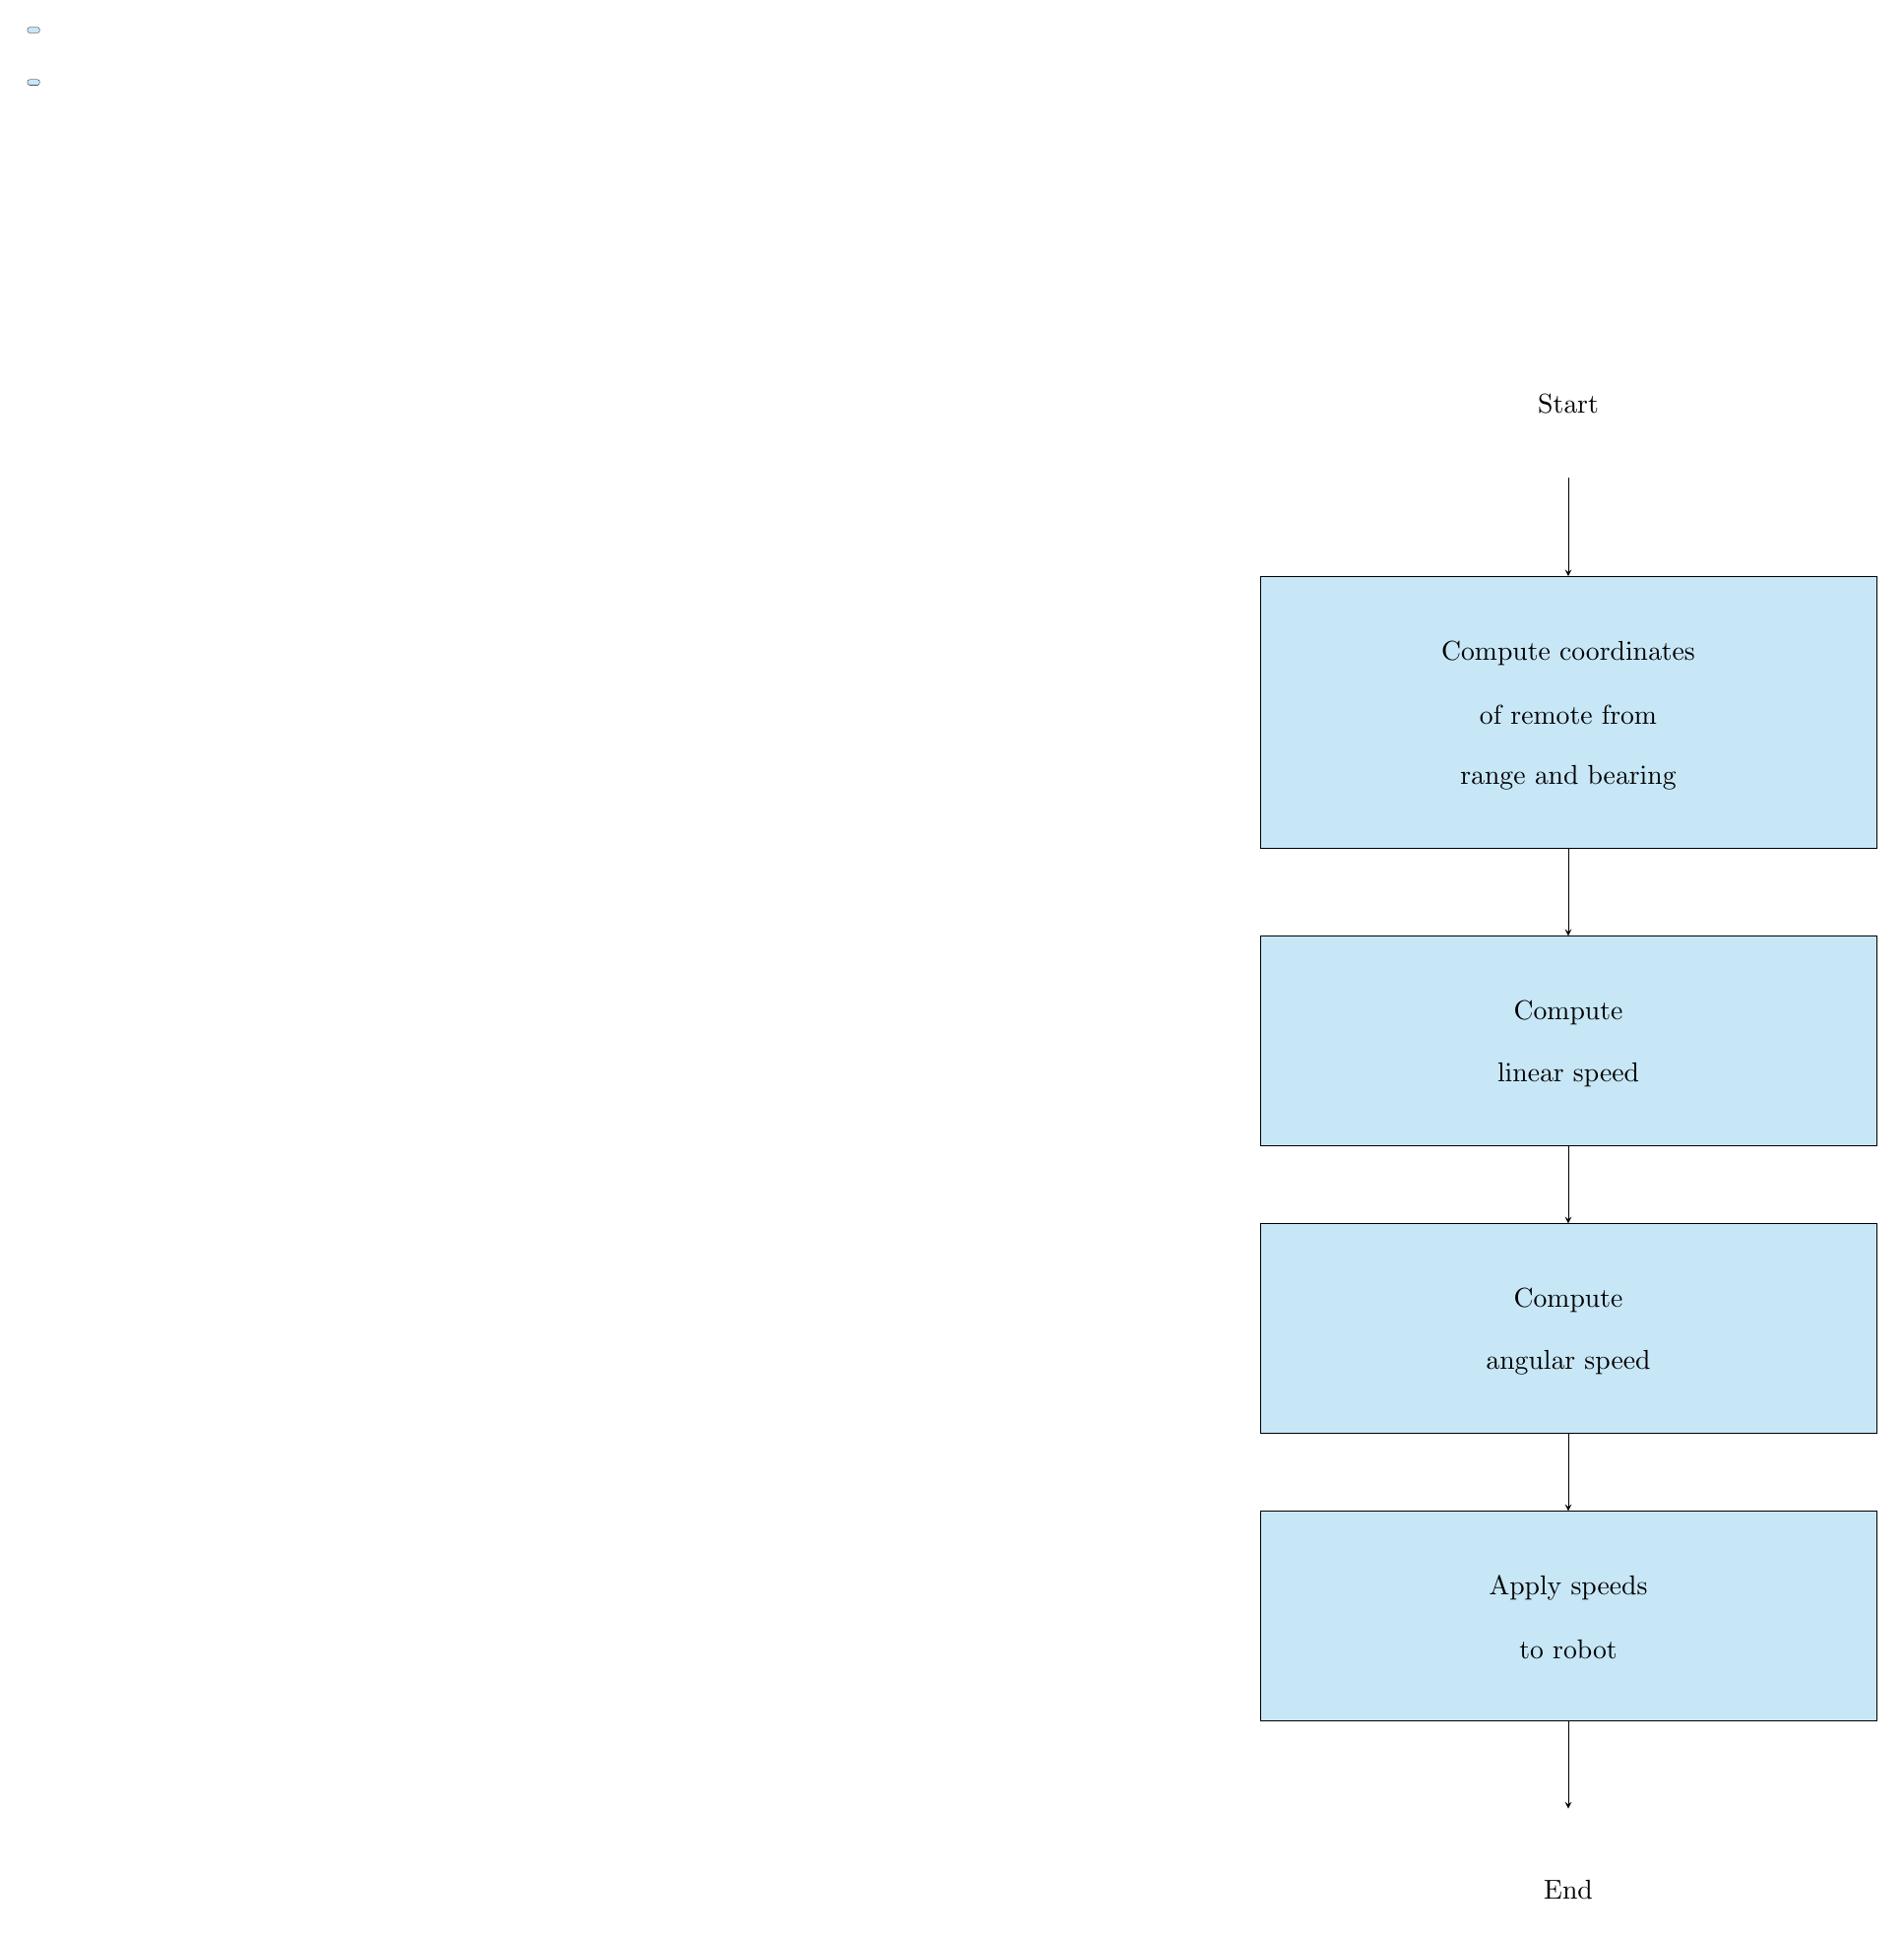
\begin{tikzpicture}
\pgftransformxscale{1.000000}
\pgftransformyscale{-1.000000}
\definecolor{dialinecolor}{rgb}{0.000000, 0.000000, 0.000000}
\pgfsetstrokecolor{dialinecolor}
\definecolor{dialinecolor}{rgb}{1.000000, 1.000000, 1.000000}
\pgfsetfillcolor{dialinecolor}
\pgfsetlinewidth{0.100000\du}
\pgfsetdash{}{0pt}
\pgfsetdash{}{0pt}
\pgfsetbuttcap
\pgfsetmiterjoin
\pgfsetlinewidth{0.100000\du}
\pgfsetbuttcap
\pgfsetmiterjoin
\pgfsetdash{}{0pt}
\definecolor{dialinecolor}{rgb}{0.780392, 0.905882, 0.968627}
\pgfsetfillcolor{dialinecolor}
\pgfpathmoveto{\pgfpoint{19.006275\du}{3.950000\du}}
\pgfpathlineto{\pgfpoint{22.032525\du}{3.950000\du}}
\pgfpathcurveto{\pgfpoint{22.450363\du}{3.950000\du}}{\pgfpoint{22.789088\du}{4.397715\du}}{\pgfpoint{22.789088\du}{4.950000\du}}
\pgfpathcurveto{\pgfpoint{22.789088\du}{5.502285\du}}{\pgfpoint{22.450363\du}{5.950000\du}}{\pgfpoint{22.032525\du}{5.950000\du}}
\pgfpathlineto{\pgfpoint{19.006275\du}{5.950000\du}}
\pgfpathcurveto{\pgfpoint{18.588437\du}{5.950000\du}}{\pgfpoint{18.249713\du}{5.502285\du}}{\pgfpoint{18.249713\du}{4.950000\du}}
\pgfpathcurveto{\pgfpoint{18.249713\du}{4.397715\du}}{\pgfpoint{18.588437\du}{3.950000\du}}{\pgfpoint{19.006275\du}{3.950000\du}}
\pgfusepath{fill}
\definecolor{dialinecolor}{rgb}{0.000000, 0.000000, 0.000000}
\pgfsetstrokecolor{dialinecolor}
\pgfpathmoveto{\pgfpoint{19.006275\du}{3.950000\du}}
\pgfpathlineto{\pgfpoint{22.032525\du}{3.950000\du}}
\pgfpathcurveto{\pgfpoint{22.450363\du}{3.950000\du}}{\pgfpoint{22.789088\du}{4.397715\du}}{\pgfpoint{22.789088\du}{4.950000\du}}
\pgfpathcurveto{\pgfpoint{22.789088\du}{5.502285\du}}{\pgfpoint{22.450363\du}{5.950000\du}}{\pgfpoint{22.032525\du}{5.950000\du}}
\pgfpathlineto{\pgfpoint{19.006275\du}{5.950000\du}}
\pgfpathcurveto{\pgfpoint{18.588437\du}{5.950000\du}}{\pgfpoint{18.249713\du}{5.502285\du}}{\pgfpoint{18.249713\du}{4.950000\du}}
\pgfpathcurveto{\pgfpoint{18.249713\du}{4.397715\du}}{\pgfpoint{18.588437\du}{3.950000\du}}{\pgfpoint{19.006275\du}{3.950000\du}}
\pgfusepath{stroke}
% setfont left to latex
\definecolor{dialinecolor}{rgb}{0.000000, 0.000000, 0.000000}
\pgfsetstrokecolor{dialinecolor}
\node at (20.519400\du,4.990000\du){Start};
\pgfsetlinewidth{0.100000\du}
\pgfsetdash{}{0pt}
\pgfsetdash{}{0pt}
\pgfsetbuttcap
\pgfsetmiterjoin
\pgfsetlinewidth{0.100000\du}
\pgfsetbuttcap
\pgfsetmiterjoin
\pgfsetdash{}{0pt}
\definecolor{dialinecolor}{rgb}{0.780392, 0.905882, 0.968627}
\pgfsetfillcolor{dialinecolor}
\pgfpathmoveto{\pgfpoint{19.006275\du}{23.110600\du}}
\pgfpathlineto{\pgfpoint{22.032525\du}{23.110600\du}}
\pgfpathcurveto{\pgfpoint{22.450363\du}{23.110600\du}}{\pgfpoint{22.789088\du}{23.558315\du}}{\pgfpoint{22.789088\du}{24.110600\du}}
\pgfpathcurveto{\pgfpoint{22.789088\du}{24.662885\du}}{\pgfpoint{22.450363\du}{25.110600\du}}{\pgfpoint{22.032525\du}{25.110600\du}}
\pgfpathlineto{\pgfpoint{19.006275\du}{25.110600\du}}
\pgfpathcurveto{\pgfpoint{18.588437\du}{25.110600\du}}{\pgfpoint{18.249713\du}{24.662885\du}}{\pgfpoint{18.249713\du}{24.110600\du}}
\pgfpathcurveto{\pgfpoint{18.249713\du}{23.558315\du}}{\pgfpoint{18.588437\du}{23.110600\du}}{\pgfpoint{19.006275\du}{23.110600\du}}
\pgfusepath{fill}
\definecolor{dialinecolor}{rgb}{0.000000, 0.000000, 0.000000}
\pgfsetstrokecolor{dialinecolor}
\pgfpathmoveto{\pgfpoint{19.006275\du}{23.110600\du}}
\pgfpathlineto{\pgfpoint{22.032525\du}{23.110600\du}}
\pgfpathcurveto{\pgfpoint{22.450363\du}{23.110600\du}}{\pgfpoint{22.789088\du}{23.558315\du}}{\pgfpoint{22.789088\du}{24.110600\du}}
\pgfpathcurveto{\pgfpoint{22.789088\du}{24.662885\du}}{\pgfpoint{22.450363\du}{25.110600\du}}{\pgfpoint{22.032525\du}{25.110600\du}}
\pgfpathlineto{\pgfpoint{19.006275\du}{25.110600\du}}
\pgfpathcurveto{\pgfpoint{18.588437\du}{25.110600\du}}{\pgfpoint{18.249713\du}{24.662885\du}}{\pgfpoint{18.249713\du}{24.110600\du}}
\pgfpathcurveto{\pgfpoint{18.249713\du}{23.558315\du}}{\pgfpoint{18.588437\du}{23.110600\du}}{\pgfpoint{19.006275\du}{23.110600\du}}
\pgfusepath{stroke}
% setfont left to latex
\definecolor{dialinecolor}{rgb}{0.000000, 0.000000, 0.000000}
\pgfsetstrokecolor{dialinecolor}
\node at (20.519400\du,24.150600\du){End};
\pgfsetlinewidth{0.100000\du}
\pgfsetdash{}{0pt}
\pgfsetdash{}{0pt}
\pgfsetbuttcap
{
\definecolor{dialinecolor}{rgb}{0.000000, 0.000000, 0.000000}
\pgfsetfillcolor{dialinecolor}
% was here!!!
\pgfsetarrowsend{stealth}
\definecolor{dialinecolor}{rgb}{0.000000, 0.000000, 0.000000}
\pgfsetstrokecolor{dialinecolor}
\draw (20.519400\du,5.950000\du)--(20.519400\du,7.217460\du);
}
\definecolor{dialinecolor}{rgb}{0.780392, 0.905882, 0.968627}
\pgfsetfillcolor{dialinecolor}
\fill (16.542550\du,7.217460\du)--(16.542550\du,10.717460\du)--(24.496250\du,10.717460\du)--(24.496250\du,7.217460\du)--cycle;
\pgfsetlinewidth{0.100000\du}
\pgfsetdash{}{0pt}
\pgfsetdash{}{0pt}
\pgfsetmiterjoin
\definecolor{dialinecolor}{rgb}{0.000000, 0.000000, 0.000000}
\pgfsetstrokecolor{dialinecolor}
\draw (16.542550\du,7.217460\du)--(16.542550\du,10.717460\du)--(24.496250\du,10.717460\du)--(24.496250\du,7.217460\du)--cycle;
% setfont left to latex
\definecolor{dialinecolor}{rgb}{0.000000, 0.000000, 0.000000}
\pgfsetstrokecolor{dialinecolor}
\node at (20.519400\du,8.207460\du){Compute coordinates};
% setfont left to latex
\definecolor{dialinecolor}{rgb}{0.000000, 0.000000, 0.000000}
\pgfsetstrokecolor{dialinecolor}
\node at (20.519400\du,9.007460\du){of remote from};
% setfont left to latex
\definecolor{dialinecolor}{rgb}{0.000000, 0.000000, 0.000000}
\pgfsetstrokecolor{dialinecolor}
\node at (20.519400\du,9.807460\du){range and bearing};
\definecolor{dialinecolor}{rgb}{0.780392, 0.905882, 0.968627}
\pgfsetfillcolor{dialinecolor}
\fill (16.542550\du,11.855470\du)--(16.542550\du,14.555470\du)--(24.496250\du,14.555470\du)--(24.496250\du,11.855470\du)--cycle;
\pgfsetlinewidth{0.100000\du}
\pgfsetdash{}{0pt}
\pgfsetdash{}{0pt}
\pgfsetmiterjoin
\definecolor{dialinecolor}{rgb}{0.000000, 0.000000, 0.000000}
\pgfsetstrokecolor{dialinecolor}
\draw (16.542550\du,11.855470\du)--(16.542550\du,14.555470\du)--(24.496250\du,14.555470\du)--(24.496250\du,11.855470\du)--cycle;
% setfont left to latex
\definecolor{dialinecolor}{rgb}{0.000000, 0.000000, 0.000000}
\pgfsetstrokecolor{dialinecolor}
\node at (20.519400\du,12.845470\du){Compute};
% setfont left to latex
\definecolor{dialinecolor}{rgb}{0.000000, 0.000000, 0.000000}
\pgfsetstrokecolor{dialinecolor}
\node at (20.519400\du,13.645470\du){linear speed};
\definecolor{dialinecolor}{rgb}{0.780392, 0.905882, 0.968627}
\pgfsetfillcolor{dialinecolor}
\fill (16.542550\du,15.564030\du)--(16.542550\du,18.264030\du)--(24.496250\du,18.264030\du)--(24.496250\du,15.564030\du)--cycle;
\pgfsetlinewidth{0.100000\du}
\pgfsetdash{}{0pt}
\pgfsetdash{}{0pt}
\pgfsetmiterjoin
\definecolor{dialinecolor}{rgb}{0.000000, 0.000000, 0.000000}
\pgfsetstrokecolor{dialinecolor}
\draw (16.542550\du,15.564030\du)--(16.542550\du,18.264030\du)--(24.496250\du,18.264030\du)--(24.496250\du,15.564030\du)--cycle;
% setfont left to latex
\definecolor{dialinecolor}{rgb}{0.000000, 0.000000, 0.000000}
\pgfsetstrokecolor{dialinecolor}
\node at (20.519400\du,16.554030\du){Compute};
% setfont left to latex
\definecolor{dialinecolor}{rgb}{0.000000, 0.000000, 0.000000}
\pgfsetstrokecolor{dialinecolor}
\node at (20.519400\du,17.354030\du){angular speed};
\definecolor{dialinecolor}{rgb}{0.780392, 0.905882, 0.968627}
\pgfsetfillcolor{dialinecolor}
\fill (16.542550\du,19.272590\du)--(16.542550\du,21.972590\du)--(24.496250\du,21.972590\du)--(24.496250\du,19.272590\du)--cycle;
\pgfsetlinewidth{0.100000\du}
\pgfsetdash{}{0pt}
\pgfsetdash{}{0pt}
\pgfsetmiterjoin
\definecolor{dialinecolor}{rgb}{0.000000, 0.000000, 0.000000}
\pgfsetstrokecolor{dialinecolor}
\draw (16.542550\du,19.272590\du)--(16.542550\du,21.972590\du)--(24.496250\du,21.972590\du)--(24.496250\du,19.272590\du)--cycle;
% setfont left to latex
\definecolor{dialinecolor}{rgb}{0.000000, 0.000000, 0.000000}
\pgfsetstrokecolor{dialinecolor}
\node at (20.519400\du,20.262590\du){Apply speeds};
% setfont left to latex
\definecolor{dialinecolor}{rgb}{0.000000, 0.000000, 0.000000}
\pgfsetstrokecolor{dialinecolor}
\node at (20.519400\du,21.062590\du){to robot};
\pgfsetlinewidth{0.100000\du}
\pgfsetdash{}{0pt}
\pgfsetdash{}{0pt}
\pgfsetbuttcap
{
\definecolor{dialinecolor}{rgb}{0.000000, 0.000000, 0.000000}
\pgfsetfillcolor{dialinecolor}
% was here!!!
\pgfsetarrowsend{stealth}
\definecolor{dialinecolor}{rgb}{0.000000, 0.000000, 0.000000}
\pgfsetstrokecolor{dialinecolor}
\draw (20.519400\du,10.717460\du)--(20.519400\du,11.855470\du);
}
\pgfsetlinewidth{0.100000\du}
\pgfsetdash{}{0pt}
\pgfsetdash{}{0pt}
\pgfsetbuttcap
{
\definecolor{dialinecolor}{rgb}{0.000000, 0.000000, 0.000000}
\pgfsetfillcolor{dialinecolor}
% was here!!!
\pgfsetarrowsend{stealth}
\definecolor{dialinecolor}{rgb}{0.000000, 0.000000, 0.000000}
\pgfsetstrokecolor{dialinecolor}
\draw (20.519400\du,14.555470\du)--(20.519400\du,15.564030\du);
}
\pgfsetlinewidth{0.100000\du}
\pgfsetdash{}{0pt}
\pgfsetdash{}{0pt}
\pgfsetbuttcap
{
\definecolor{dialinecolor}{rgb}{0.000000, 0.000000, 0.000000}
\pgfsetfillcolor{dialinecolor}
% was here!!!
\pgfsetarrowsend{stealth}
\definecolor{dialinecolor}{rgb}{0.000000, 0.000000, 0.000000}
\pgfsetstrokecolor{dialinecolor}
\draw (20.519400\du,18.264030\du)--(20.519400\du,19.272590\du);
}
\pgfsetlinewidth{0.100000\du}
\pgfsetdash{}{0pt}
\pgfsetdash{}{0pt}
\pgfsetbuttcap
{
\definecolor{dialinecolor}{rgb}{0.000000, 0.000000, 0.000000}
\pgfsetfillcolor{dialinecolor}
% was here!!!
\pgfsetarrowsend{stealth}
\definecolor{dialinecolor}{rgb}{0.000000, 0.000000, 0.000000}
\pgfsetstrokecolor{dialinecolor}
\draw (20.519400\du,21.972590\du)--(20.519400\du,23.110600\du);
}
\end{tikzpicture}

  \caption{Flowchart of Navigation Algorithm}
  \label{fig:navAlgoFlowchart}
\end{figure}

\begin{algorithm}[h!]
  \SetAlgoLined
  \KwIn{Range $d_{ref}$ and Bearing $\theta_{ref}$ of Remote}
  \KwOut{Mobile Robot Trajectory}
  Constants: following distance $d_f$ and proportional gains $K_p$ and $K_\omega$\\
  \Begin
  {
    Compute target point with respect to robot's local frame as $x_{ref} = (d_{ref} - d_f)\cos \theta_{ref}$, $y_{ref} = (d_{ref} - d_f)\sin \theta_{ref}$\\
    Compute linear speed $v(t) = sign(x_{ref})K_p\sqrt{x_{ref}^2 + y_{ref}^2}$\\
    Compute $\omega(t) = K_\omega \theta_{ref}$\\
    Apply wheel speeds to robot\\
  }
  \caption{Navigation Algorithm}
  \label{alg:navAlgo}
\end{algorithm}

% \subsection{Specifications}

% \section{Preliminary Work}

% \subsection{Modelling} \label{sec:model}

% \subsection{Simulation Results} \label{sec:simresults}

% \subsection{Design} \label{sec:design}

% \subsection{Experimental Activities} \label{sec:expresults}


% \section{Parts List}

\section{Timeline and Milestones} \label{sec:timeline}

\begin{figure}
  \centering
  \begin{ganttchart}[
    hgrid,
    vgrid,
    x unit=.6cm,
    y unit title=.8cm,
    y unit chart=.6cm,
    milestone label font=\tiny,
    milestone progress label font = \tiny,
    milestone progress label anchor = east,
    bar label font=\tiny,
    group label font=\small,
    bar/.append style={fill=green},
    bar incomplete/.append style={fill=red},
    group progress label font = \tiny,
    progress label text={$\displaystyle#1\%$},
    group progress label anchor = east,
    bar progress label font = \tiny,
    bar progress label anchor = east,
    ]{1}{17}

    \gantttitle{2020}{17}\\
    \gantttitle{Sep}{4}
    \gantttitle{Oct}{4}
    \gantttitle{Nov}{4}
    \gantttitle{Dec}{4}
    \gantttitle{}{1}\\

    \ganttgroup[progress = 100]{Research}{3}{12} \\
    \ganttbar[progress = 100]{Research Multipath}{3}{12}\\
    \ganttbar[progress = 100]{Research Reflector}{3}{12}\\

    \ganttgroup[progress = 80]{Simulation}{8}{10}\\
    \ganttbar[progress = 80]{CoppeliaSim simulation}{8}{10}\\
    \ganttmilestone[progress = 0]{Simulation Complete}{10}\\

    \ganttgroup[progress = 100]{Project Proposal}{11}{12}\\
    \ganttbar[progress = 100]{Proposal Document}{11}{11}\\
    \ganttbar[progress = 100]{Proposal Presentation}{12}{12}\\

    \ganttgroup[progress = 82.5]{XBee Setup}{13}{14}\\
    \ganttbar[progress = 90]{Voltage Regulator Circuit}{13}{13}\\
    \ganttbar[progress = 80]{Configuration with X-CTU}{14}{14}\\
    \ganttbar[progress = 90]{Sensing RSSI}{14}{14}\\
    \ganttbar[progress = 70]{Serial Communication}{14}{14}\\
  \end{ganttchart}
\caption{Gantt chart for Fall 2020}
\label{fig:gantt1}
\end{figure}

\begin{figure}
  \centering
  \begin{ganttchart}[
    hgrid,
    vgrid,
    x unit=.6cm,
    y unit title=.8cm,
    y unit chart=.6cm,
    milestone label font=\tiny,
    milestone progress label font = \tiny,
    milestone progress label anchor = east,
    bar label font=\tiny,
    group label font=\small,
    bar/.append style={fill=green},
    bar incomplete/.append style={fill=red},
    group progress label font = \tiny,
    progress label text={$\displaystyle#1\%$},
    group progress label anchor = east,
    bar progress label font = \tiny,
    bar progress label anchor = east,
    ]{1}{18}
    \gantttitle{2021}{18}\\
    \gantttitle{Jan}{2}
    \gantttitle{Feb}{4}
    \gantttitle{Mar}{4}
    \gantttitle{Apr}{4}
    \gantttitle{May}{4}\\

    \ganttgroup[progress = 0]{Assembly}{3}{4}\\
    \ganttbar[progress = 0]{Replace Motors}{3}{3}\\
    \ganttbar[progress = 0]{Design and Construct Reflector}{3}{4}\\
    \ganttbar[progress = 0]{Mount Reflector}{4}{4}\\
    \ganttmilestone[progress = 0]{Assembly Complete}{4}\\

    \ganttgroup[progress = 10]{Software}{5}{6}\\
    \ganttbar[progress = 20]{XBee Library}{5}{5}\\
    \ganttbar[progress = 0]{Control Library}{6}{6}\\

    \ganttgroup[progress = 0]{Angle Estimation}{7}{8}\\
    \ganttbar[progress = 0]{Rotate XBee on Stepper Motor}{7}{7}\\
    \ganttbar[progress = 0]{Determine Angle}{8}{8}\\

    \ganttgroup[progress = 0]{Distance Estimation}{9}{10}\\
    \ganttbar[progress = 0]{Calibrate Distance Calculation}{9}{10}\\

    \ganttgroup[progress = 0]{Subsystem Integration}{11}{15}\\
    \ganttbar[progress = 0]{Angle Estimation Testing}{11}{11}\\
    \ganttbar[progress = 0]{Distance Estimation Testing}{12}{13}\\
    \ganttbar[progress = 0]{System Testing}{14}{15}\\
    \ganttmilestone[progress = 0]{Integration Complete}{15}\\

    \ganttgroup[progress = 0]{Project Completion}{16}{17}\\
    \ganttbar[progress = 0]{Final Report}{16}{16}\\
    \ganttbar[progress = 0]{Final Presentation}{17}{17}\\
    \ganttbar[progress = 0]{Presentation to IAB}{17}{17}\\
    \ganttbar[progress = 0]{Project Demo}{17}{17}\\

    \ganttmilestone[progress = 0]{Project Complete}{17}
  \end{ganttchart}
  \caption{Gantt Chart for Spring 2020}
  \label{fig:gantt2}
\end{figure}

The Gantt charts in Figures \ref{fig:gantt1} and \ref{fig:gantt2} show our planned schedule to complete this project. In these charts, there are four sections in each month represented by the dotted grid. This is to approximate a weekly schedule. Our first milestone is to complete the simulation of the system in MATLAB and CoppeliaSim. This includes simulating a remote as well as the robotic cart. The simulation of the RSSI detection will be handled in Matlab based on the positions of the cart and remote. We will add noise to the simulated RSSI in order to simulate the multipath effect. The expected functionality is that the cart will follow the remote.

The second milestone is to complete the assembly of both the cart and the remote. The cart assembly involves replacing the existing motors with the purchased motors, as well as mounting the stepper motor, reflector, and XBee on top of the robot. The assembly of the remote involves constructing the voltage regulator circuit.

The third milestone is to integrate the subsystems into one system. This will involve testing the angle and distance estimation from the cart to the remote. It will also include testing the following capabilities of the overall system. We expect that this will require a large amount of debugging and tuning. Therefore, we have allotted several weeks for this purpose.

The fourth and final milestone is to complete the final report and presentation. This involves documenting our findings in a report and presenting our work. At this point, the project will be complete.

\section{Concluding Remarks}
A robotic cart that follows the user is a useful application of mobile robotics. Although some methods of performing this task have been developed, the existing methods require line-of-sight sensing between the robot and the cart. Our proposed robotic cart system does not require line-of-sight since it uses analog wireless signal strength as opposed to ultrasonic or photographic sensing. In this way, we plan to develop a robotic cart that can detect the user even in the presence of obstacles.

\pagebreak
\bibliographystyle{IEEEtran}
\bibliography{bib/references.bib}

\end{document} 

%%% Local Variables:
%%% mode: latex
%%% TeX-master: t
%%% End:
